\documentclass[11pt]{article} % do not change this line
\input{BigDataStyle.txt}      % do not change this line
\usepackage{amsmath,amsfonts,amssymb,amsthm,latexsym,graphicx}
\usepackage{pdfpages}
\usepackage{algorithm}
\usepackage{algorithmicx}
\usepackage{minted}
\usepackage[noend]{algpseudocode}

\emergencystretch=5mm
\tolerance=400
\allowdisplaybreaks[4]

\theoremstyle{plain}
\newtheorem{theorem}{Theorem}[section]
\newtheorem{proposition}[theorem]{Proposition}
\newtheorem{corollary}[theorem]{Corollary}
\newtheorem{lemma}[theorem]{Lemma}
\newtheorem{problem}[theorem]{Problem}

\theoremstyle{definition}
\newtheorem*{remark}{Remark}

\title{Evaluating distributed time synchronization for musical applications using Ableton Link}
\author{Xavier Riley}

\newcommand{\Programme}{Distributed and Networked Systems}

\begin{document}
\maketitle

\declaration

% assessment criteria
% - synchronization accuracy under various delays
% - message complexity/bandwidth
% - difficulty of setup/integration (useability)
% - failure modes/spof? (f failures, failure of leader)
% - resilience to drift (how often do we resync?)
% - available topologies, effect on performance (ideally constant with diameter of graph)

% Ableton Live
% - aims, tradeoffs, assumptions (reliable network)
% - works via multicast, discovery, exchanging timelines
% - fault tolerance concepts (sending on all changes)
% Can it be improved upon without violating simplicity? To provide:
% - resilience to lost messages (reliable broadcast) - does it already do this?
% - resistance to crash faults (simple consensus) - protocol assumes a shared network - not sure this makes sense
% - improvements in synchronization bounds - what are the current limits? - are they perceptible? (within 10ms)
% - other things I haven't considered yet

% Possible experiment criteria
% We can't measure things like dropped writes or stale reads so what are the
% criteria for a music system? Draw comparisons with gossip analysis -
% convergence time, stability, resilience to pertubations. Also check how clock
% sync literature handles this.
% The main thing is that the tempo stays in sync for as much time as possible

% What your project *must* contain
% motivations and original aims including how this work may help in future career
% assessment inc. self evaluation. How did it go? What did you do right or
%      wrong? What have you learnt about planning and execution? Where next?

% should contain
% - abstract
% - introduction
% - background research (literature survey/review)
% - either

% sofware product - software engineering method, requirements analysis, design,
% implementation, testing - also user or installation manual

% theoretical - development of theory, inc small programs, explanation of
% algorithms, descriptions of hard theory, results, analysis

% experimental - experimental results, analysis, conclusions

% - professional issues (as appendix - c. 1000 words)
% - self assessment
% - bibliography
% - any code, including instructions on how to run
% - other - layout diagrams, sample output, program listing

\begin{abstract}
  With the recent explosion of connected musical devices, the challenge of
  making these play "in time" with each other mounts against application
  developers and device manufacturers. Ableton Link\cite{goltz2018ableton} aims
  to provide robust musical synchronization using principles from distributed
  systems programming, in contrast to previous master/slave approaches. However
  the evaluation criteria for such a system are not well represented in the
  existing literature, with particular reference to a musical context.  The
  following presents a system for empirical testing of the Ableton Link library
  using the Jepsen\cite{jepsen} testing framework, along with a set of criteria
  for evaluating similar libraries that may be developed in future.
\end{abstract}

% Motivations
%
% Artistic output but also, music industry is large and $$$
% requirements of a musical performance
% - ensemble
% - timekeeping (layers - a year is one orbit of the sun, a day one rotation on the earths' axis)
% - colocated as opposed to geo-distributed
% clock synchronization literature
% - internal, external, pulse based - how have these been applied to music so far? Which work well?
% distributed systems and music
% - what distinguishes music from the rest of the clock synchronization
%   literature?
% - music (and clock sync) is not linear data! Consistency is not the primary issue. If a peer drifts or goes out of time,
%   it doesn't create merge problems. It can simply restart and all is well. Largely stateless
% - the challenge is mainly keeping tight synchronization bounds for as much time as possible
% - also practical challenges around the experience for those using the software
% - there are *some* consistency issues though. For example, synchronizing on current tempo and other transport messages

\section{Introduction}

The synchronizing of events is fundamental to our perception of musical
performance. Where performers are using networked connected devices, the
challenge maintaining accurate synchronization incorporates the well studied
problem of clock synchronization from distributed systems.

This work examines the Ableton Link\cite{goltz2018ableton} protocol, which
appears to be one of the first attempts at applying concepts from distributed
computing to the problem of musical synchrony. Through empirical testing it is
shown to maintain a reasonable degree of consistency under adverse network
conditions. This work also examines the impact of asymmetric network delays on
the clock synchronization algorithms in use by the protocol. Bandwidth usage is
also analysed and found to be higher on the leader in connected topologies,
although data transfer in absolute terms is relatively low.

It is also proposed that the presence of a non-monotonic clock offset may
introduce inconsistencies within rounds, however the regular retransmission of
state means that the session will converge eventually provided there are no
permanent network partitions.

This project has allowed me to develop practical skills in the area of testing
distributed network protocols. It is my hope that this proves to be useful in
my future professional work with distributed systems more generally. The
frameworks (Jepsen\cite{jepsen} in particular), methodologies and background
research have all informed my outlook so far and I will continue to investigate
some of the related areas after this project is finished.

\section{Project goals and methodology}

The aim of this project is to establish a set of criteria to evaluate
distributed solutions to the problem of musical synchronization. Using these
criteria as a benchmark, we then evaluate whether a specific solution is viable
for reliable music production and performance. The benefits of such a system
are evident (robust to node failures/dropouts, simplified set up) - this work
instead aims to examine some of the potential pitfalls when running such a
system under conditions that simulate commodity network hardware.

In examining a single system, Ableton Link, it is hoped that the criteria and
testing methodology will prove useful for future research into alternative
distributed solutions.

\subsection{Evaluating synchronization for music systems}

With the advent of distributed systems for music applications, there are
natural questions around how these should be assessed to determine their
effectiveness. Traditional criteria from distributed systems research may be
useful, particularly around the bounds for timing synchronization, however
musical performance doesn't have the same requirements as traditional
databases, for example. A musical tempo can diverge and converge again with
only minor consequences, however avoiding a double spend for a bank account
requires more careful treatment.

This means that bounds for synchronization and notions of data consistency may
be relaxed if doing so would benefit some other aspect, such as ease of
setup/integration.

\subsection{Fundamental problems of music synchronization}

To characterize some of the challenges more specifically, the following list
covers some of the key criteria for success:

\begin{itemize}
  \item Getting clocks in sync \cite[Chapter~6.3.2]{attiya2004distributed}
  \item Keeping them in sync (in the presence of drift or variable latency) \cite[Chapter~13]{attiya2004distributed}
  \item Network bandwidth (ensuring scalability as number of devices grows)
  \item Fault tolerance % (master availability, *musical* consistency, convergence time)
  \item Ease of setup and deployment
\end{itemize}

\section{Background research}

As network technologies continue to grow in usage and importance to musical
performances\cite{madgwick2015simple}, it becomes increasingly important to
find common approaches to allow devices and applications to synchronize, without
reliance on expensive proprietary technology or protocols which are difficult to
implement and configure. The need to purchase or to understand such equipment
creates an unnecessary barrier to entry, potentially impeding important
contributions from musicians who lack the necessary financial or educational
resources.

\subsection{About Ableton Link}

Ableton Link is an open source, permissively licensed C++ library for
integration with application code. As well as the popular digital audio
workstation Ableton Live, implementations exist for a large number of mobile
applications and for many of the popular music programming environments. In
addition the following three design goals are stated\cite{goltz2018ableton}:

\begin{itemize}
  \item Remove the restrictions of a typical master/client system
  \item Remove the requirement for initial setup
  \item Scale to a wide variety of music applications
\end{itemize}

It differs from existing approaches in that it does not rely on a master
process to propagate timing information directly. Instead nodes will establish
a session, using a reference to the start time of the oldest member of the
group even if that member is no longer present.

Clock synchronization is performed using a Kalman filter which adds a level of
robustness to jitter introduced by network delays, along with a more accurate
reflection of the real delay under certain conditions. This approach appears to
be relatively sophisticated when compared with other music programs using basic
averaging algorithms such as NTP\cite{bletsas2005evaluation}.

Implementation is handled by application developers who are left to integrate a
small API. C++ has widespread support for integration with many popular
languages, making this viable for the majority of existing applications.

Setup for the end user is virtually transparent - network discovery takes place
automatically on all interfaces. Clock synchronization is performed
automatically for nodes joining a session and then at 30 second intervals
afterwards. Simple transport commands (start, stop) and tempo changes are also
propagated automatically by reliable broadcast.

Failures, drop outs and re-entry are all handled with a model of eventual
consistency where last-write-wins takes effect for changes in tempo and
transport state.

\subsection{Alternative software solutions}

Music programming environments in the academic space are well catered for with
regards to open source software, however applications in the consumer market
have tended to lag behind some of these advances. Often either the production
of music is limited to a single device, or additional devices are synchronized
using specialized hardware dedicated to synchronizing frames e.g. MIDI, SMTPE -
see Goltz\cite{goltz2018ableton} for a review of these methods.

The use of networks in computer music is an active area of study, with much of
the research being driven by "laptop orchestras"\cite{trueman2007laptop}
centred around academic institutions. This has led to widespread adoption of
the Open Sound Control
protocol\cite{wright2005open}\cite{madgwick2015simple}\cite{narveson2013landini}
as the "lingua franca" of connected musical applications.

Ableton Link uses a custom network protocol but all networking is handled via
private methods within the library, meaning that application developers
choosing to implement it do not need to concern themselves with network level code.

\subsection{Co-located vs. Geo-distributed}

When considering the synchronization of musical programs and important
distinction is whether the participants are "within earshot" of each other. If
performers are distributed across a large geographic distance, such that they
could not reasonably hear the audible output of their peers, then staying
within the thresholds of tolerable latency starts to become impossible. This
means that performers cannot react to each other in a normal way due to the
effect of lag.

The position taken in this work is that geo-distributed performance is more a
matter of maintaining a locally consistent ordering of events and relative
timings rather than accurate synchronization, and as such is not under the
scope of discussion here.

Other works have taken a different view, attempting to offer creative solutions
to overcome the inherent latency with wide-area communication. In
Oda\cite{oda2017tools} these include the use of GPS timing to provide a
globally consistent time server, along with predictive instruments that attempt
to send messages to remote clients to synthesize a performer's actions ahead of
time in order to overcome latency. While interesting, in their current state
these are unlikely to be generalizable to consumer software.

Focusing on co-located performance, the prime objective becomes to achieve and
maintain synchrony between devices. Secondary concerns include maximum
convergence time on any relevant notions of shared state, e.g. tempo,
start/stop times.

\subsection{Finding bounds - the limits of human perception}

In order to determine some lower and upper bounds on the level of synchrony
required, data gathered around musical perception will be useful. While the
consensus is not complete\cite{greeff2016influence}, one can assume that
musical performers can tolerate up to 40ms of latency between sources. This is
of course dependent on the individual performer as well as other factors such
as the frequency domain of the sound.

In addition to delays that impact live performers, any delay introduces the
risk of comb filtering effects on sound from multiple sources. This occurs when
the frequencies from once sound source reinforce or cancel out those from
another sound source.

Finally, the accurate synchronization of multiple speakers is essential for the
use of sound spatialization effects, such as stereo panning or surround sound.

With these in mind, the lower bound would ideally be zero (perfect
synchronization) but this is unlikely in practice. Delays of 0.05ms could
theoretically introduce comb filtering effects in the audible frequency range
at 10kHz\cite{lester2007effects} so this may offer a more practical lower bound.

In terms of an upper bound, 40ms of delay would appear to be the upper limit in
terms of the impact on the majority of listeners. Where human performers are
involved, this is more likely to impact their ability to play, so a lower
figure of 20ms may be more appropriate\cite{chafe2004network}.

\subsection{Prior testing approaches}

LANdini\cite{narveson2013landini} was designed for use with a specific laptop
orchestra in mind and was "tested" in rehearsal and performance. Functional
testing is also described in their paper regarding reliability of message
delivery and bandwidth usage.

A more rigorous testing scheme is proposed in the development of
PiGMI\cite{Oda2016} (The Raspberry Pi Global Metronome) in which metronome
pulses were produced by the synchronized device at 120 pulses per minute for a
duration of 30 minutes. The output is then recorded into separate channels on a
sound card and later analysed to determine offsets. In addition to this,
commercial drum machines were also measured, synchronized using MIDI time
clock, to add a benchmark.

This method of testing allows for excellent accuracy measuring "time at
speaker" which is arguably the most realistic metric available; However, the
recording, analysis methods and the reliance on physical hardware makes
replication of results more challenging.

A similar result may be achieved using virtual audio inputs on a single machine
e.g. using the Soundflower application on OS X, however such solutions are
subject to their own sources of latency. In addition, testing within a single
machine in this way would not allow for detecting drift in the system clock,
relative to real time, if additional reference time sources are not also used.

\section{Evaluation Criteria and Experiment Design}

The system will be judged by the following criteria:

\begin{center}
\begin{tabular}{|c|l|}
 \hline
  Musical consistency & convergence of nodes under tempo changes \\
  \hline
  Bandwidth & how many messages are required by the protocol \\
  \hline
  Network Topologies & performance under different network layouts \\
  \hline
  Delay distributions & effect of latency distributions on synchronization\\
 \hline
\end{tabular}
\end{center}

These are defined in more detail below.

The testing approach taken in this work chooses not to measure the audio output
but instead analyses the reported times from each of the application nodes for
each beat at the current tempo which should occur at the same time across all
nodes. This approach allows for a simple reproduction of results and a more
flexible way to test different failure modes and network conditions.

This is achieved using the Jepsen framework\cite{jepsen}, which was
originally designed to test safety guarantees under fault injection, however it
is also flexible enough to test systems with less strict guarantees.

The framework starts five instances running a simple Ableton Link application
inside Linux containers using Docker. In addition to these, a control node is
started which invokes and records operations against the existing nodes.
Primarily this is concerned observing stability and consistency under read and
write operations against the tempo parameter of the Link session.

The Jepsen framework also allows the control node to introduce faults into the
virtual network between the nodes. Under initial conditions they are all
connected, however links between nodes can be cut (packets between nodes all
dropped) to form different topologies. Variable or fixed latency can also be
introduced. These take place via a process called a "nemesis" in the framework
terminology.

The format of the test is as follows: nodes are started and allowed to join the
session automatically. The control node then sequences a cycle of read, write,
write operations on the tempo field with a random tempo between 20 and 220
representing the usual range of musical tempos. These operations are performed
on a randomly selected node, spaced at an interval of 2 seconds apart. This
continues for 60 operations totalling around 180 seconds. This figure was
picked to correspond to the traditional 3 minute pop song.

Each node also logs its state at each beat (see Algorithm 1), the placement of
the beat being determined by the Link protocol. These are then analysed
following the test to calculate the offsets and convergence of events following
changes in tempo.

This approach could be criticised as being less accurate - the processing time
can introduce variations such that the status is not printed exactly on the
beat - however this is more typical of the usage in a real world
implementation. In measuring convergence (described below) the log analysis
groups the status output from all nodes to within a 100ms window to account for
any variations due to processing times. The maximum tempo used in this test is
240 beats per minute which has an inter-beat interval of 250ms, larger than the
uncertainty window in use.

The alternative would be to calculate the status output at the point of the
next beat. This was trialled, however changes from faster to slower tempi
caused occurrences where the next beat at a slower tempo would have occurred
before the current beat at a faster tempo, causing entries to go "back in
time". These discontinuities in the timeline were clearly unrealistic and
calculating the next beat from a given point in time would have introduced
unnecessary complexity to the testing procedure.

\makeatletter
\def\BState{\State\hskip-\ALG@thistlm}
\makeatother

\begin{algorithm}
  \caption{Test procedure}\label{linktest}
\begin{algorithmic}[1]
\BState \emph{loop}:
\State \textbf{print} {$\textit{status}()$};
\State \textbf{sleep} {$\textit{time-until-next-beat}()$};
\State \textbf{goto} \emph{loop}.
\end{algorithmic}
\end{algorithm}

\subsection{Consistency in a musical context} \label{musicalConsistency}

The introduction of faults and perturbations to the network can cause nodes to
receive updates late, resulting in divergence for the beat markers in the
session. Ableton Link aims to provide eventual
consistency\cite{vogels2009eventually} provided the network remains free of
partitions so these should recover in time.

This leads to an interesting question of how to quantify the divergence and the
resulting effect on the music. This work puts forward that Ableton Link and
similar eventually consistent systems in future should measure "musical
consistency" as the time spent in agreement relative to the length of the
overall session.

\begin{figure}
  \caption{Example of divergent time measurements}
  \centering
  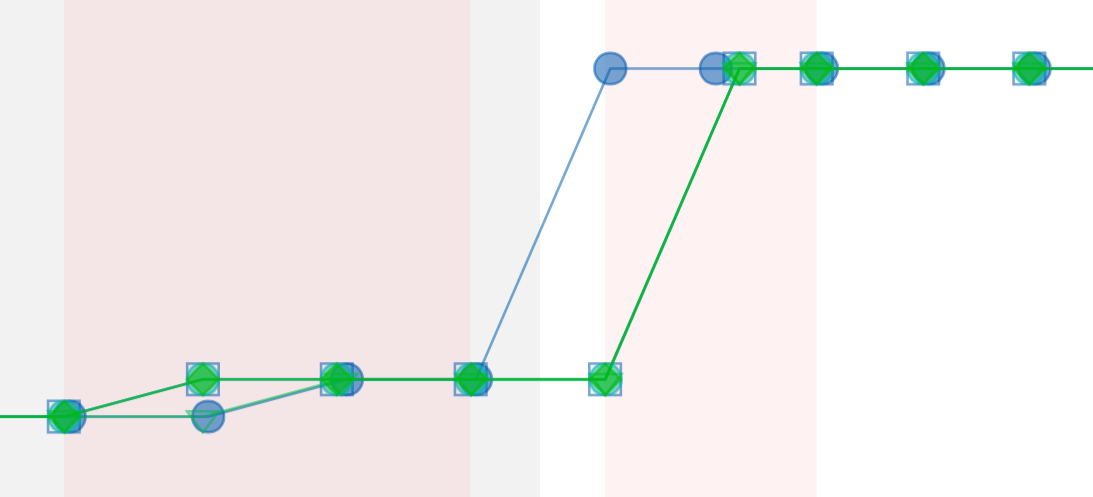
\includegraphics[width=0.75\textwidth]{figures-for-publication/musical-consistency-example.png}
  \label{fig:divergence-example}
\end{figure}

In the accompanying results the periods of inconsistency are highlighted in
pink. Figure \ref{fig:divergence-example} shows an example where a single node has
received a tempo update before this could be propagated to the other peers,
causing it to move early. Convergence following such an event is judged as the
first read operation for which all nodes are present and within an error bound
of 100ms.  This error bound is used as some degree of smoothing is necessary to
counteract natural variance in the measurements being taken.

The duration of these divergence periods is summed and divided by the total
session time to give a percentage relative to the length of the session.

\begin{figure}
  \caption{Musical consistency calculation}
  \centering
  \begin{equation}\label{eqn:musical-consistency}
    musical\;consistency=\frac{\sum divergence\;period\;durations}{session\;duration}
  \end{equation}
\end{figure}

This could be viewed as a variant on Time-based staleness proposed by Bermbach
et al \cite{bermbach2013towards} with a simplification to allow for an easier
comparison between sessions of similar lengths.

\subsection{Synchronization Accuracy versus Bandwidth}

In order to combat clock drift, some synchronization systems will allow a high
frequency of synchronization events to ensure greater accuracy. This comes at
the expense of more messages being sent over the network. For example, the
LANdini project opts for 3 synchronization messages (pings) every second.

For comparison, recent work by Geng et al\cite{geng2018} achieves
synchronization on the order of 10s of nanoseconds within datacenters, however
around 5 MBits/s of bandwidth is used to achieve this result.

Given that Ableton Link targets a mass market, the use of consumer grade
routers should be assumed. This makes it important to minimize the number of
messages sent by the protocol to avoid overloading the hardware, while striving
for the figures set out in tolerable latency above.

The synchronization protocol of Link is not documented, however from analysis
of the codebase it can be seen that clock synchronization events take place
when a new peer is discovered, and then at 30 second intervals thereafter.

This involves the sending of at least 50 outbound messages and receiving at
least 50 inbound messages under the default settings (these are not
currently configurable via a public interface). Assuming a successful run every
30 seconds with no rejected messages, this works out at 3.33 messages per
second on average.

\subsection{Use of Jepsen, Docker and log parsing}

While Jepsen is primarily designed to exercise safety guarantees of distributed
systems under partitions, the flexibility it offers allows for different kinds
of tests to be performed. This work opts mainly to use Jepsen to handle the
running of tests and fault injection, whereas the analysis of results takes
place in a separate process which handles the parsing of log files generated
during the test.

The use of Docker containers allows straightforward reproducibility across all
major platforms. One possible application would be in a continuous integration
(CI) testing environment so that changes to the Link codebase could be
exercised against these tests automatically.

As the Link protocol favours transparent setup over configuration, there is a
limited about of information available regarding the state of the session by
default. For these tests, the debug logging in the Link library is enabled and
these logs are then parsed following the test to produce the output in the
results section below.

\subsection{Topologies and latencies}

As part of the stated aim of ease of setup, the Ableton Link protocol performs
service discovery and message broadcast on all network interfaces to ensure
that all connected nodes are able to join the same session. For example, nodes
using a LAN may also see other nodes on a WiFi network provided that at least
one node existed that was connected to both.

This feature introduces the prospect of topologies other than a connected
network in practice. Jepsen allows different topologies to be defined and
implemented during the test procedure. As Link operates using a type of
reliable broadcast algorithm (retransmitting the state of the session on all
interfaces when a valid state update is received) the topologies may be ranked
according to the length of the maximum diameter of the network over which an
update can be propagated.

\begin{itemize}
  \item Connected
  \item Bridge
  \item Line
\end{itemize}

Another test condition concerns the performance of the protocol under small,
constant network delays. In the tests below this is defined as 48ms delays on
all nodes except the leader for reasons outlined below.

The protocol is also exercised in the presence of larger delays (500ms). The
timings for these are included on the charts below.

Finally, differing distributions of delays are examined as follows:

\begin{itemize}
  \item Constant delay
  \item Normal distribution
  \item Pareto distribution
\end{itemize}

\section{Analysis}

\subsection{Note on the visual formatting of results}

The visual output from the tests contains a variety of information which will
be described as follows. Appendix \ref{appendix:experimental-results} contains
graphical plots of the results obtained during the test runs.

Each page shows an single test run. The upper graph charts the current tempo (y
axis) from each peer on each musical beat (equivalent to time, x axis). The
lower chart shows the clock offset measurements from the leader of the group
The lower chart shows the clock offset measurements from the leader of the
group - the tests are constructed such that node \textit{n1} is always started
first and is therefore the leader for the session. The offset measurements are
then between \textit{n1} and each of the remaining 4 nodes \textit{n2, n3, n4}
and \textit{n5}.

The sections coloured grey represent the "nemesis" regions - these are the
times during which the network conditions (topologies and latencies) are
applied.

The sections coloured in pink mark "divergence periods" as explained in section
\ref{musicalConsistency}. These give an added visual indication for periods in
which the nodes do not agree on the current tempo and/or beat timings.

\subsection{Musical Consistency}

The results are summarized in the following table:

\begin{center}
\begin{tabular}{|c|c|c|c|c|c|}
 \hline
  \multicolumn{4}{|c|}{Musical consistency} \\
 \hline
  delay & connected & bridge & line\\
 \hline
  0ms & 98.644\% & 96.212\% & 96.942\%\\
  48ms constant & 89.858\% & 91.571\% & 90.385\%\\
  48ms normal & 89.17\% & 93.432\% & 95.088\%\\
  48ms pareto & 100.0\% & 97.77\% & 97.833\%\\
  500ms constant & 91.538\% & 82.199\% & 89.134\%\\
  500ms normal & 90.207\% & 84.946\% & 90.48\%\\
  500ms pareto & 97.062\% & 94.346\% & 96.13\%\\
 \hline
\end{tabular}
\end{center}

These show that the Link protocol is generally resilient to different network
conditions. No test run observed any major divergence and musical consistency
was generally good under the zero delay and pareto conditions.

There was considerable difficulty in obtaining precise measurements given the
lack of configuration options and very little in the way of callbacks,
especially regarding clock synchronization. This may account for some of the
variation, however the graphs reflect that for the most part, 5 nodes were
maintaining synchrony.

\subsection{Effects of delay distributions on clock synchronization}

In order to simulate network delays of various types the Jepsen framework uses
the NetEm (network emulation) module as part of the Traffic Control package on
Linux\cite{hemminger2005network}. This allows for outgoing packets from a node
to be delayed by a given amount, according to different statistical
distributions.

\begin{itemize}
  \item constant - each packet is delayed by a fixed amount
  \item normal - packets are delayed by a Gaussian distribution centred on the given time
  \item pareto - given time parameter defines the duration over which a long tail distribution is calculated.
\end{itemize}

Of these, the pareto distribution is the most similar to the self-similar
"heavy tail" delays found in real-world WiFi
networks\cite{bletsas2005evaluation}\cite{zhang2008delay}, however the constant
and normal distributions are useful indicators for other types of network
conditions. For example, in \cite{wang2014improving} delays to secondary users
caused by interference (contention) are linear with respect to their distance
from the access point.  More constant delays are therefore useful to indicate
the performance of Ableton Link for the lower bounds of latency under these
kinds of conditions.

The Ableton Link library code contains an undocumented upper limit on clock
synchronization round trip times: Any measurement which takes longer than 50ms
will be rejected and retried. If more than 5 measurement packets (again, an
undocumented limit) are "in flight" during the run of measurements, the run
will be cancelled for that round. The process will then wait for the next 30
second interval to pass before attempting to synchronize again.


\begin{figure}
  \caption{Clock offset measurement failures}
  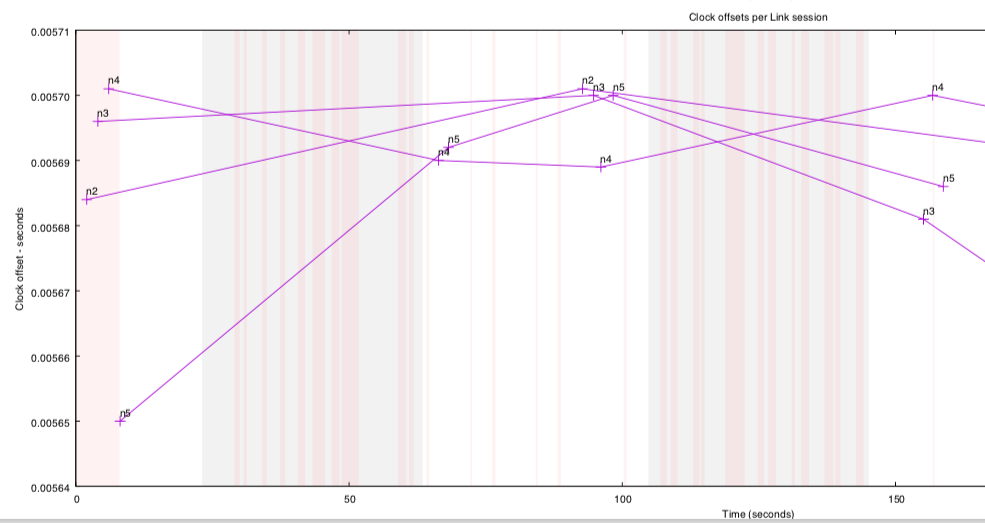
\includegraphics[width=1\textwidth]{figures-for-publication/offset-measurement-failures.png}
  \label{fig:offset-measurements-missed}
\end{figure}

This means that any sustained period of delays above 50ms will result in
synchronization measurements not being taken. This can be seen in
Figure ~\ref{fig:offset-measurements-missed} showing the 500ms delay condition - no
synchronization events occur in the grey shaded areas which represent the delay
conditions being applied. Exceptions to this occur in the results when the
testing framework is not able to execute the traffic shaping command on a node
at the start of a nemesis period.

\subsection{Symmetric and asymmetric delays}

For delays below the 50ms RTT threshold, clock synchronization events will
still take place, however the clock synchronization algorithm does not reflect
the presence of delays in cases where both the forward path (leader) and
the reverse path (peer) have delays to their outbound packets. This is because
a symmetric delay will centre around a measurement of zero (or the original
offset as if no delay were present).

\begin{figure}
  \caption{Clock offset under asymmetric delay}
  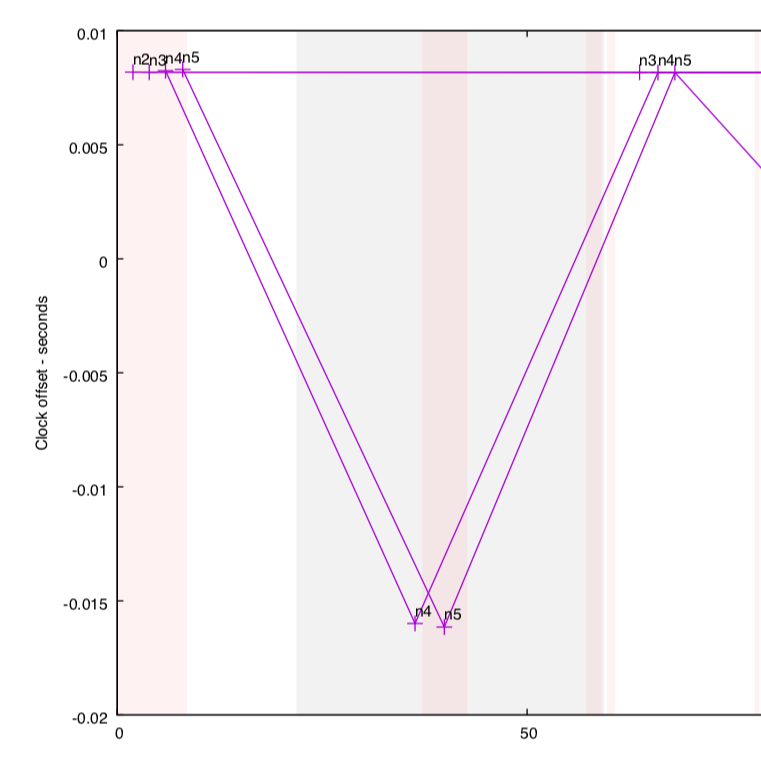
\includegraphics[width=1\textwidth]{figures-for-publication/clock-offset-example.png}
  \label{fig:delayExample}
\end{figure}

Aside from being a source of confusion during early investigation, this is
actually a desirable condition in Ableton Link; The point at which peers are
judged to be synchronized is their "time at speaker" and given that the local
computation related to timestamping events does not require network calls then
any offset introduced by network latency should (ideally) not be taken into
account.

Introducing an asymmetric delay in the tests on all peers except the leader
causes synchronization events to be offset by half of the given delay time. In
the examples above this is typically around 25ms negative offset for the 50ms
one-way delay. This is illustrated in Figure \ref{fig:delayExample} where the delay
condition (shaded grey on the graph) caused the offset measurements for nodes 4
and 5 to move from around +8ms to around -16ms when the asymmetric delay is
applied. Nodes 2 and 3 failed to complete their offset measurements in this
case due to the 50ms timeout that the Link protocol imposes.

Placing the asymmetric delay on the leader only causes the
offset to "flip" to a 25ms positive offset. This would be seen as
a movement from the typical offset of between 5-7ms (it is suggested that
this is a result of processing overheads in the containers) to an offset of
around +30ms.

\subsection{Bandwidth usage and message complexity}

Using the logging features of the iptables program, the number of packets sent
between nodes during a test run (connected network, no delay) are shown as
follows:

\begin{center}
\begin{tabular}{|c|c|c|c|c|c|}
 \hline
  \multicolumn{6}{|c|}{Packet count / Bandwidth} \\
 \hline
  from/to &  n1 (leader) & n2 & n3 & n4 & n5\\
 \hline
  n1 & "-/-" & 1829/236K & 1823/235K & 1822/235K & 1826/236K\\
  n2 &1826/225K & "-/-" & 1502/203K & 1498/202K & 1504/203K\\
  n3 &1818/224K & 1500/203K & "-/-" & 1492/201K & 1498/202K\\
  n4 &1814/224K & 1493/202K & 1489/201K & "-/-" & 1491/201K\\
  n5 &1816/224K & 1497/202K & 1493/202K & 1488/201K & "-/-"\\
 \hline
\end{tabular}
\end{center}

Here we see that the leader (n1) handles roughly 17.5\% more than the other
peers in the connected case with no delays applied. This is because the Ableton
Link library will prefer a connection to the leader during a clock
synchronization event. If the leader is not accessible from the peer, the next
neighbouring peer ordered by ID is chosen.

This does raise a theoretical concern with regards to scalability as the leader
handles proportionally more traffic, however in practice the group is unlikely
to reach a size required to cause stability issues in a local network.

Comments in the codebase indicate that future work to choose a synchronization
peer based on the local topology are being considered.

\subsection{Resilience during periods of packet loss}

The design of Ableton Link opts for UDP messaging throughout. Somewhat
surprisingly for a system without a reliable messaging layer like TCP, the Link
protocol maintains musical consistency under conditions of heavy packet loss.
This may be in part due to the high level of redundancy in broadcasting updates
- each node will re-broadcast the relevant state changes after receiving a
"newer" event containing a change to the local state. In addition, each node
will broadcast state at 5 second intervals. At the expense of some bandwidth,
this approach does appear to have merit when looking at the results of the tests.

\subsection{Comments on mutable timelines and temporary divergence}

A number of applications that rely on timing do so using the system clock.
While this is relegated to being an implementation detail in the literature,
there is a growing agreement in the software engineering community that using
the system clock is an unreliable source for measuring elapsed time, in part
due to it's mutability. This has been the source of a number of major software
outages and failures\cite{monotonic}.

A proposed method which offers a reliable alternative for measuring elapsed
time is the use of monotonic clocks. This are based on a monotonically
increasing counter and have the desirable property that they will never be
adjusted backwards or run at an artificially fast or slow rate, unlike system
clocks under the control of NTP or similar synchronization methods.

Monotonic clocks are used by Ableton Link\cite{goltz2018ableton} to avoid such
issues. This is important because the ordering of events and the election of a
leader in a session are determined using timestamps. Using a mutable source of
timestamps such as the system clock would affect the ability of the system to
maintain correct ordering.

In addition to peers maintaining their own monotonic clock timestamp, the clock
synchronization process determines additional offsets (deltas) relative to the
leader of the session. Unlike the monotonic counter however, these offsets are
necessarily mutable and can have the effect of moving a node "back in time"
relative to another peer.

\begin{algorithm}
  \caption{Temporary Divergence}\label{linkdivergence}
\begin{algorithmic}[1]
\item{ }
\end{algorithmic}
\end{algorithm}

\begin{minted}{ruby}
# Ping/pong measurement has hardcoded cap of 50ms for RTT
# Assuming RTT / 2 for latency calculation, this allows
# for a deviation of +/-25ms either side of leader

# Node A - @nodeA.delta == 25ms
@nodeA.set_tempo(120)
@nodeA.bcast({:tempo => 120, :global_host_time=> (99.975 + 0.025)})
# clock synchronization event - @nodeA.delta == 0m
@nodeA.set_tempo(140)
@nodeA.bcast({:tempo => 140, :global_host_time=> (99.975 + 0.0)})
# 140 is set locally (timestamp not checked for local updates)

# Node B
@nodeB.receive({:tempo => 120, :global_host_time => 100.0}) do
  if received_global_host_time > current_tempo.global_host_time
    @nodeB.set_tempo(received_tempo)
    @nodeB.bcast({:tempo => received_tempo,
                  :global_host_time => received_global_host_time})
  end
end

# 120 has a higher global host time
# 140 is therefore rejected, introducing temporary inconsistency

@nodeA.receive({:tempo => 120, :global_host_time => 100.0})
# this is newer that the timestamp for @nodeA's current tempo,
# therefore @nodeA will adopt it

# If @nodeA.receive(120) is dropped or lost when received by
# @nodeC, then @nodeC will adopt 140 as the tempo, however it
# should still converge.
\end{minted}

Normally conditions such as these might pose a major issue to the consistency
of the protocol, however eventually consistency is usually restored as state is
broadcast at regular 5 second intervals (effectively rounds) and on subsequent
state updates. This means that the agreement on tempo among the session is
unlikely to diverge for more than 5 seconds.

Even so, this inter-round divergence is an area that would need attention if
this protocol were to be adapted to environments with more strict requirements
e.g. factory/warehouse automation.

At the expense of an increase in message size, a potential solution to this
issue is offered by Hybrid Logical Clocks\cite{kulkarni2014logical} proposed by
Kulkarni et al.

\begin{algorithm}
  \caption{Tempo changes with Hybrid Logical Clocks}\label{linkhlc}
\begin{algorithmic}[1]
\item{ }
\end{algorithmic}
\end{algorithm}

\begin{minted}{ruby}
# Node A - @nodeA.delta == 25ms, @nodeA.logical_time = 0
@nodeA.set_tempo(120) # @nodeA.lt += 1
@nodeA.bcast({:tempo => 120,
              :logical_time => 1,
              :counter => 0,
              :global_host_time=> (99.975 + 0.025)})
# clock synchronization event - @nodeA.delta == 0m
@nodeA.set_tempo(140) # @nodeA.lt += 1
@nodeA.bcast({:tempo => 140,
              :logical_time => 2,
              :counter => 0,
              :global_host_time=> (99.975 + 0.0)})

# Node B - @nodeB.logical_time = 0
#        - @nodeB.global_host_time = 100.1
@nodeB.receive({:tempo => 120,
                :logical_time => 1,
                :counter => 1,
                :global_host_time => 100.0}) do
  @nodeB.logical_time = max([self.logical_time,
                             received_logical_time,
                             self.global_host_time])

  if self.logical_time.unchanged? && \
     self.logical_time == received_logical_time
    self.counter = max(self.counter, received_counter) + 1
  elseif self.logical_time.unchanged?
    self.counter = self.counter + 1
  elseif self.logical_time == received_logical_time
    self.counter = received_counter + 1
  else
    self.counter = 0
  end

  @nodeB.set_tempo(received_tempo)
  @nodeB.bcast({:tempo => received_tempo,
                :logical_time => 100.1,
                :counter => 0,
                :global_host_time => received_global_host_time})
end

# on receipt of tempo 140 at time 100.2
# ...
@nodeB.bcast({:tempo => received_tempo,
              :logical_time => 100.2,
              :counter => 0,
              :global_host_time => received_global_host_time})
# ...
\end{minted}

Here the timestamp on the receiving peer allows for a causal ordering meaning
that the later message is adopted.

\section{Further work}

% further ideas - even better internal sync (at the cost of bandwidth) - Google paper
% resettable oscillators - more naturally maps onto how humans synchronize perhaps
% options for geo-distributed time synchronization
% extensions beyond music to other time sensitive domains

The testing of distributed systems techniques applied to musical
synchronization would primarily benefit from more systems to test against!
Using the measures and techniques offered in this work it is hoped that an
objective comparison with future libraries may be made.

Returning focus to Ableton Link, the testing approach may form the basis of
some usable integration testing. In particular the use of containers (and
Jepsen) to provide a reproducible testing environment is being adopted as part
of a development workflow by several distributed systems such as Cockroach
DB\cite{cockroach}. Combining this testing approach with the method of
recording audio from each peer would allow for more objective measurements to
be made with regard to clock synchronization.

Given the opportunity, it would be interesting to examine alternative
techniques for clock synchronization that better accommodate asymmetric delays
and also that take account of the network topology. One example would be the
use of "coded probes" suggested by Geng et al\cite{geng2018} - by sending
timing packets from server \textit{i} to \textit{j} in pairs with a known delay
\textit{s} between them, on being received at server \textit{j} and the
interval can reflect the presence of delays in transmission. As delays are
often random in nature, the intervals closest to \textit{s} can be used to
increase accuracy.

Another area of interest would be to examine this work in the context of
related fields, one in particular being factory automation, which requires
synchronization between independent moving objects. Some of the approaches used
in the Link library may be of use in such systems however there may be
additional work required around the level and types of consistency that the
library offers.

\section{Conclusions}

From the analysis performed in this work and anecdotally working with Link on
other software projects I have found it to be an elegant, well designed and
well implemented solution to an interesting set of problems. Studying clock
synchronization in the context of musical applications offers a practical
introduction to the wider field, without the additional requirements in
expertise that often come with analysing in the context of data storage
systems.

\bibliographystyle{plain}
\bibliography{bibliography}

\appendix
\section{Experimental results}
\label{appendix:experimental-results}

% no delays
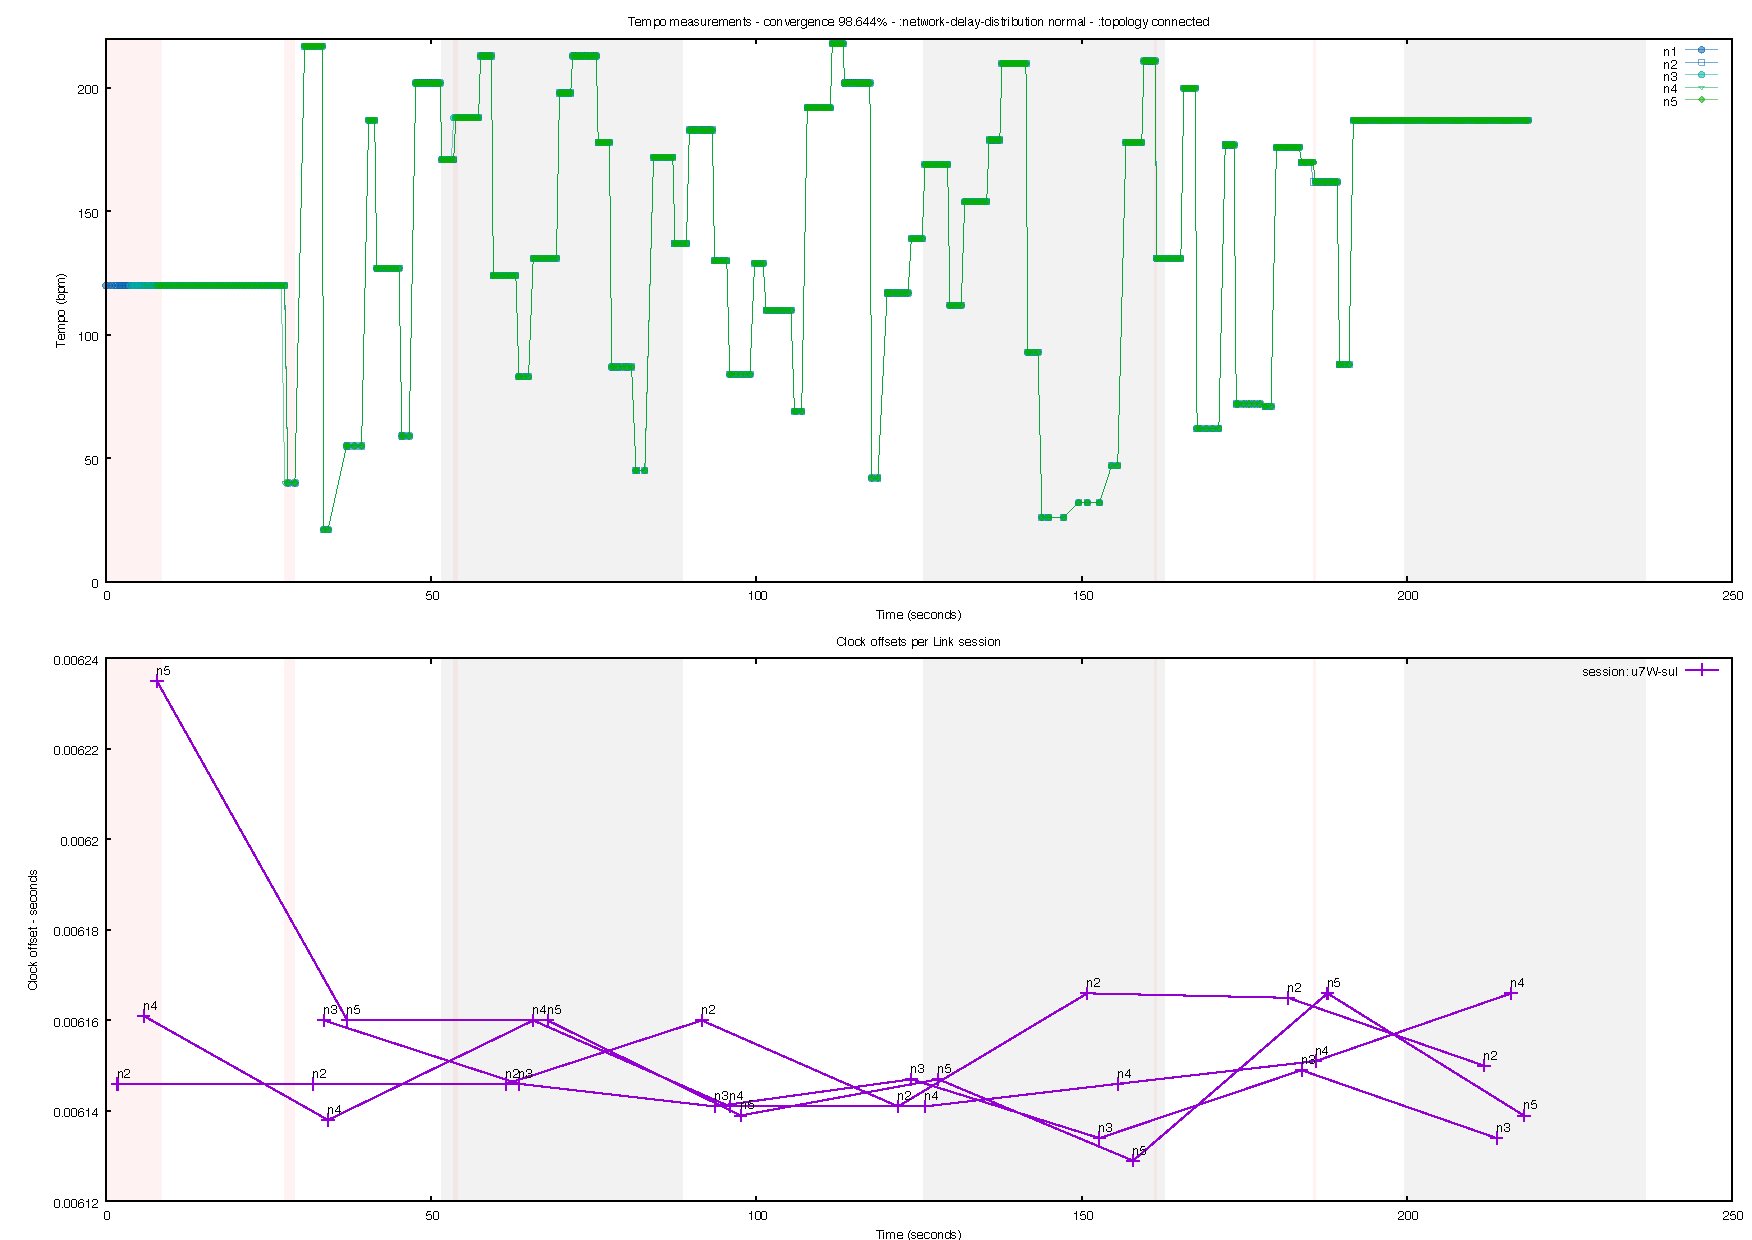
\includepdf[pages=-,angle=-90]{figures-for-publication/tempo_measurements_convergence_98_644_network_delay_distribution_normal_topology_connected/plot.pdf}
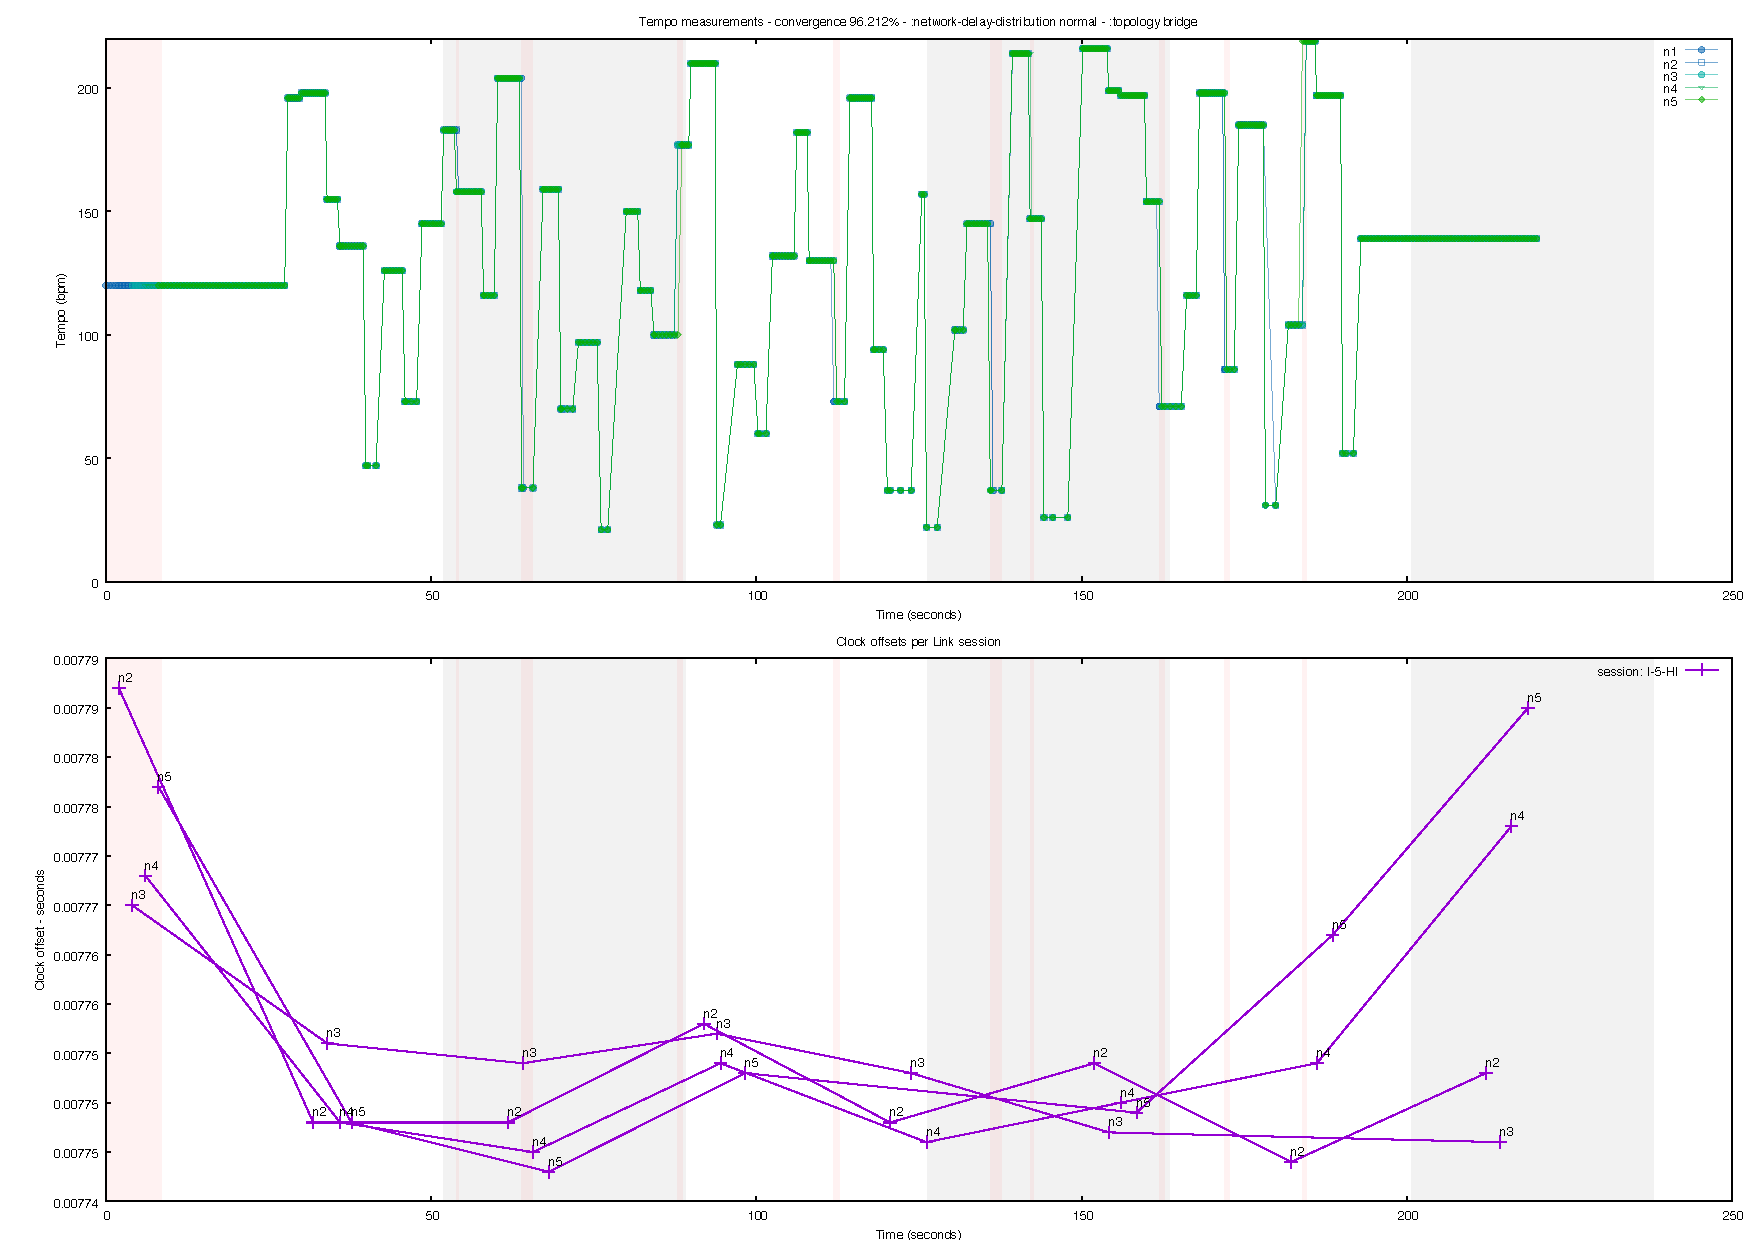
\includepdf[pages=-,angle=-90]{figures-for-publication/tempo_measurements_convergence_96_212_network_delay_distribution_normal_topology_bridge/plot.pdf}
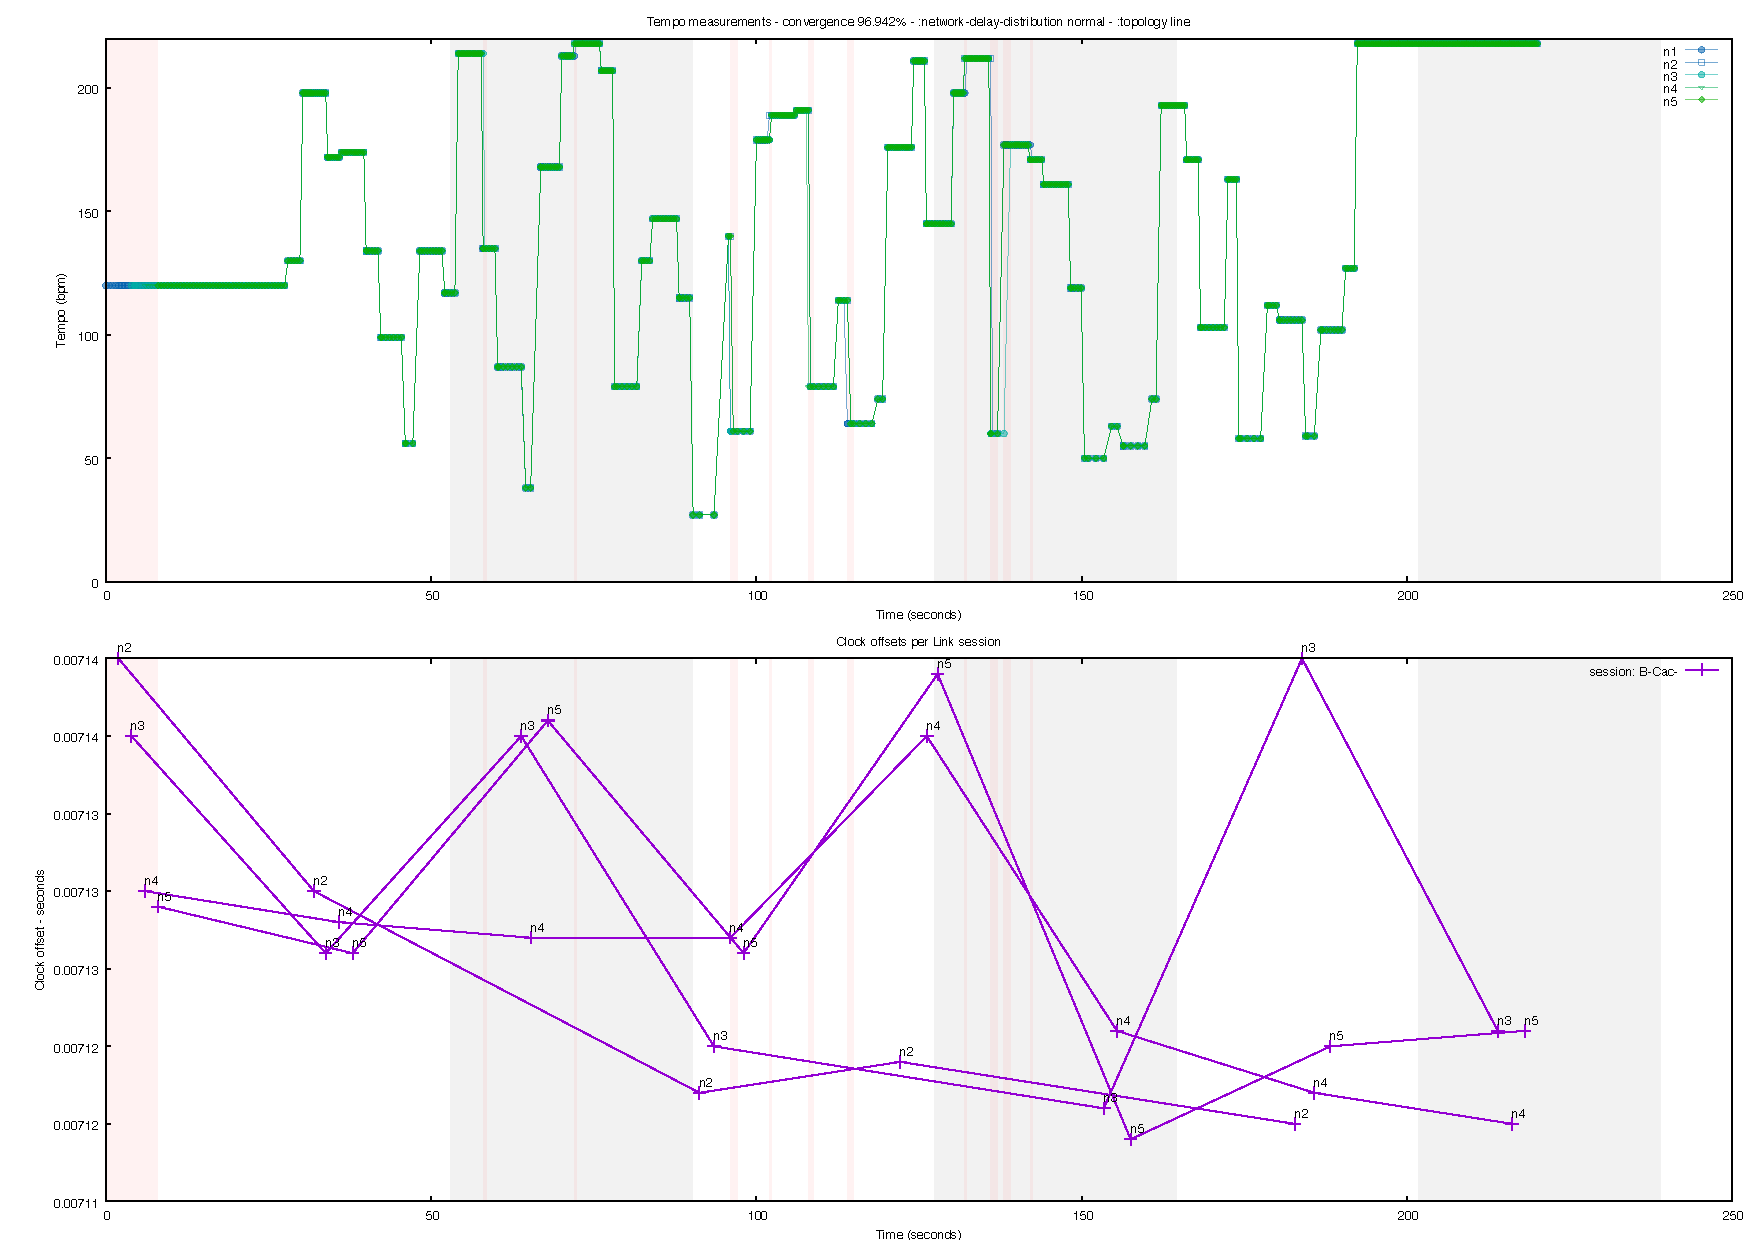
\includepdf[pages=-,angle=-90]{figures-for-publication/tempo_measurements_convergence_96_942_network_delay_distribution_normal_topology_line/plot.pdf}

% 48ms delays
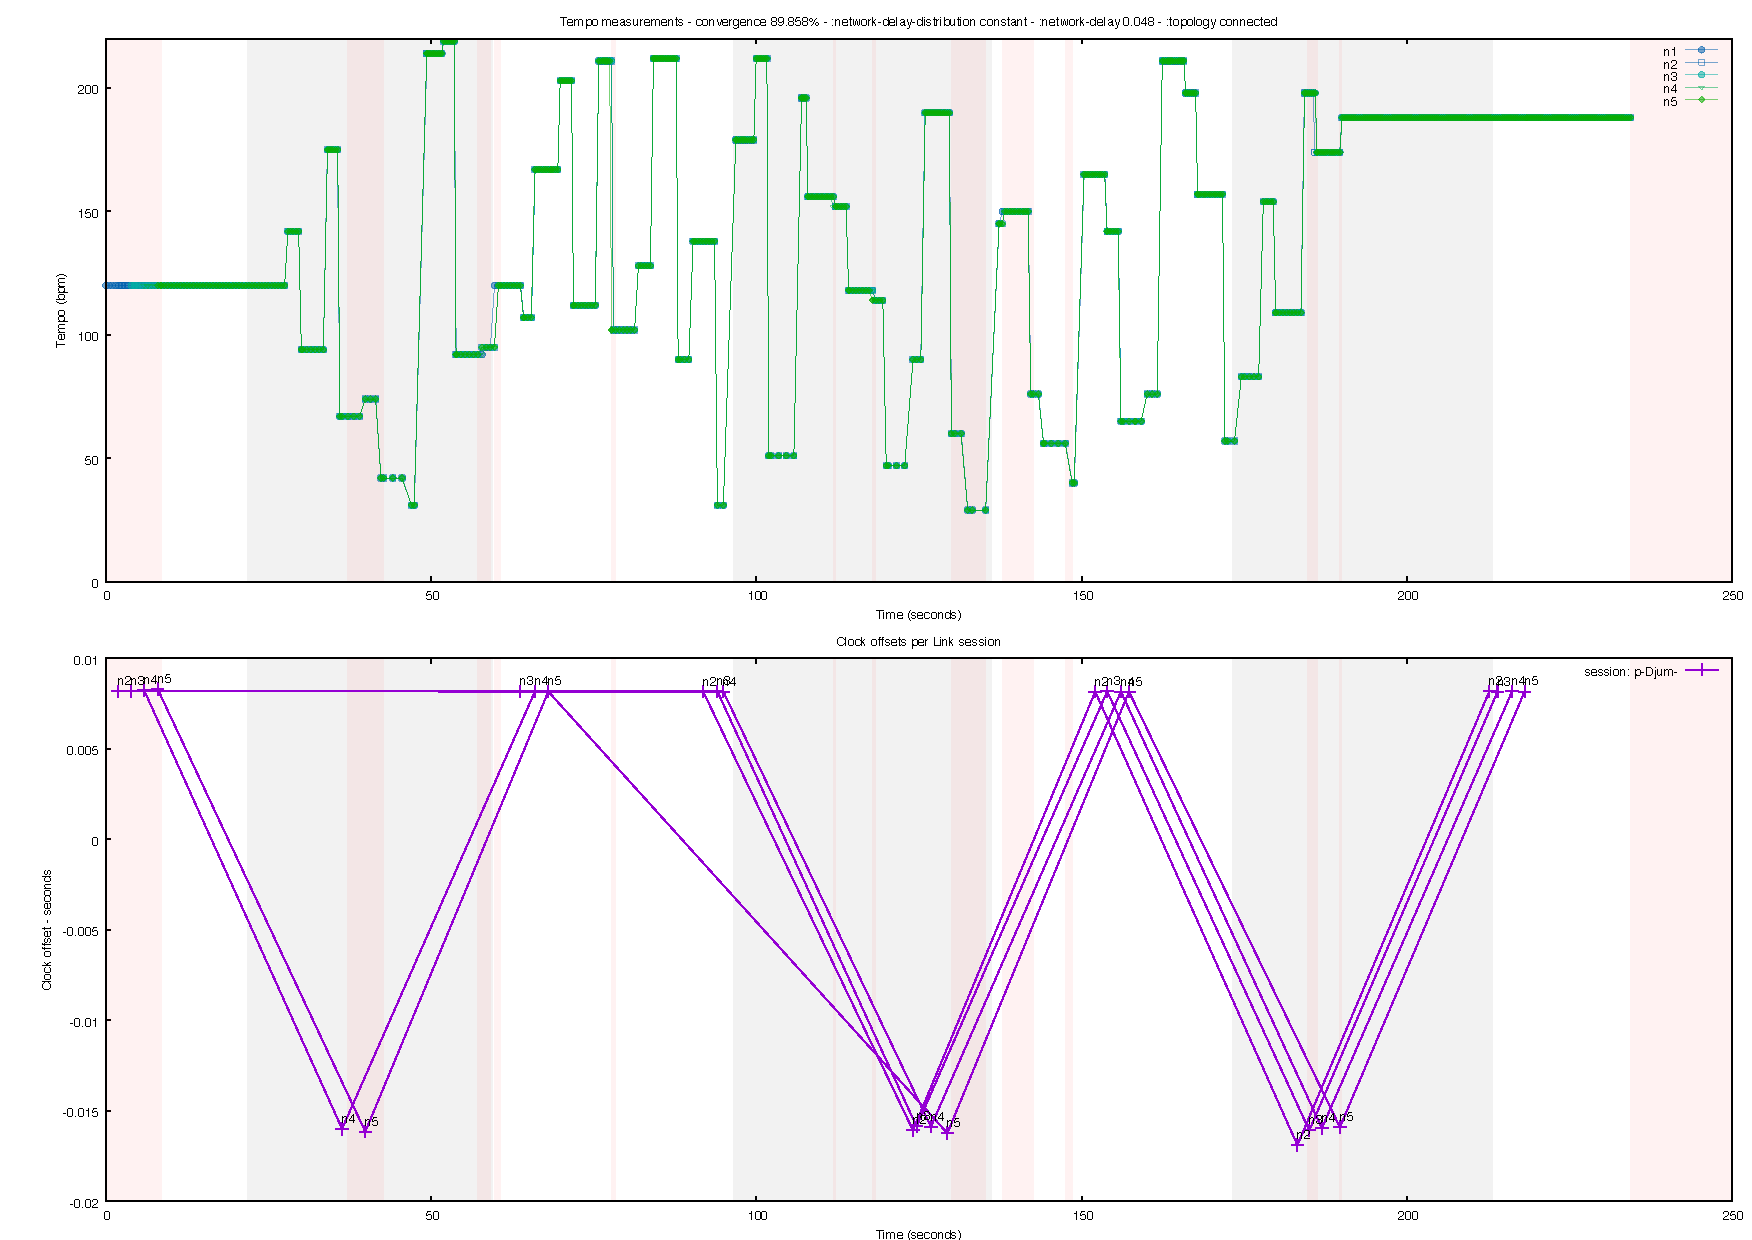
\includepdf[pages=-,angle=-90]{figures-for-publication/tempo_measurements_convergence_89_858_network_delay_distribution_constant_network_delay_0_048_topology_connected/plot.pdf}
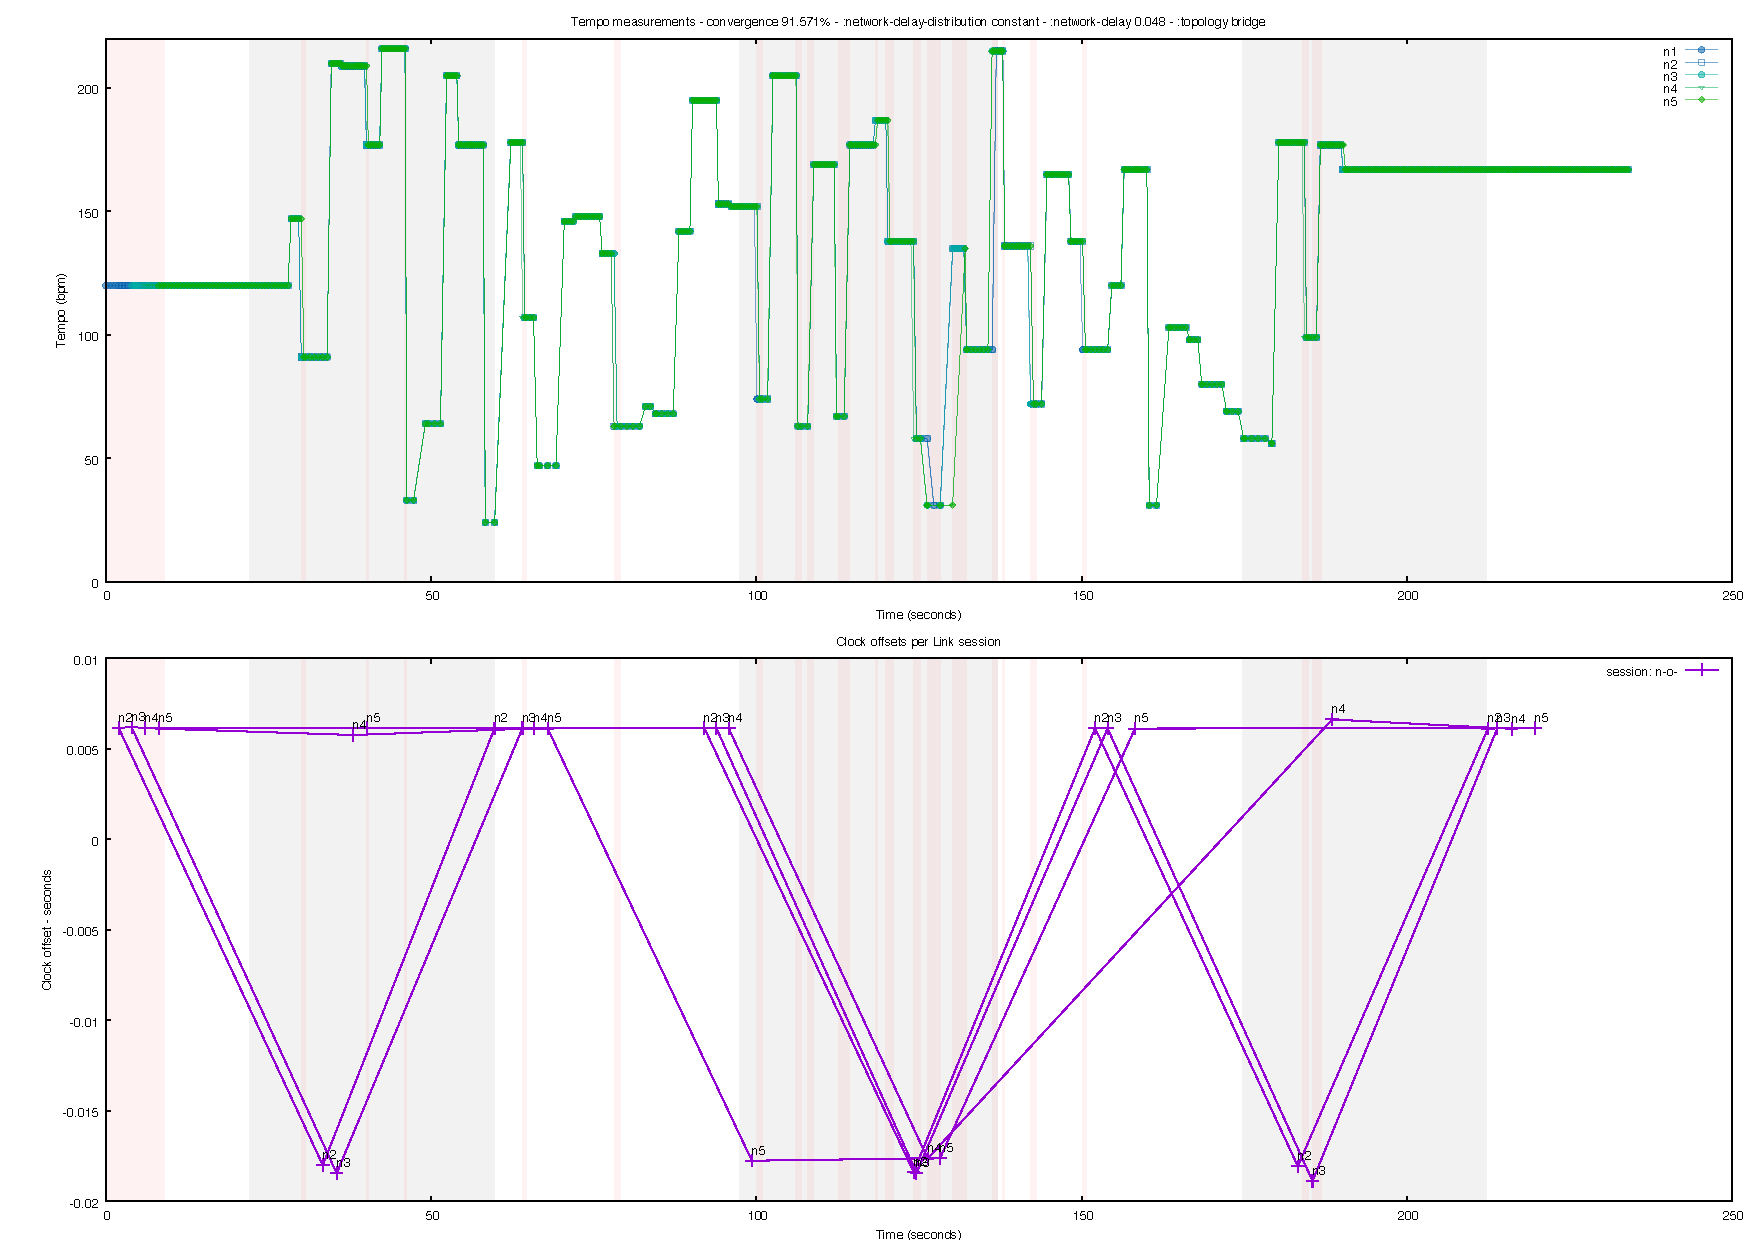
\includepdf[pages=-,angle=-90]{figures-for-publication/tempo_measurements_convergence_91_571_network_delay_distribution_constant_network_delay_0_048_topology_bridge/plot.pdf}
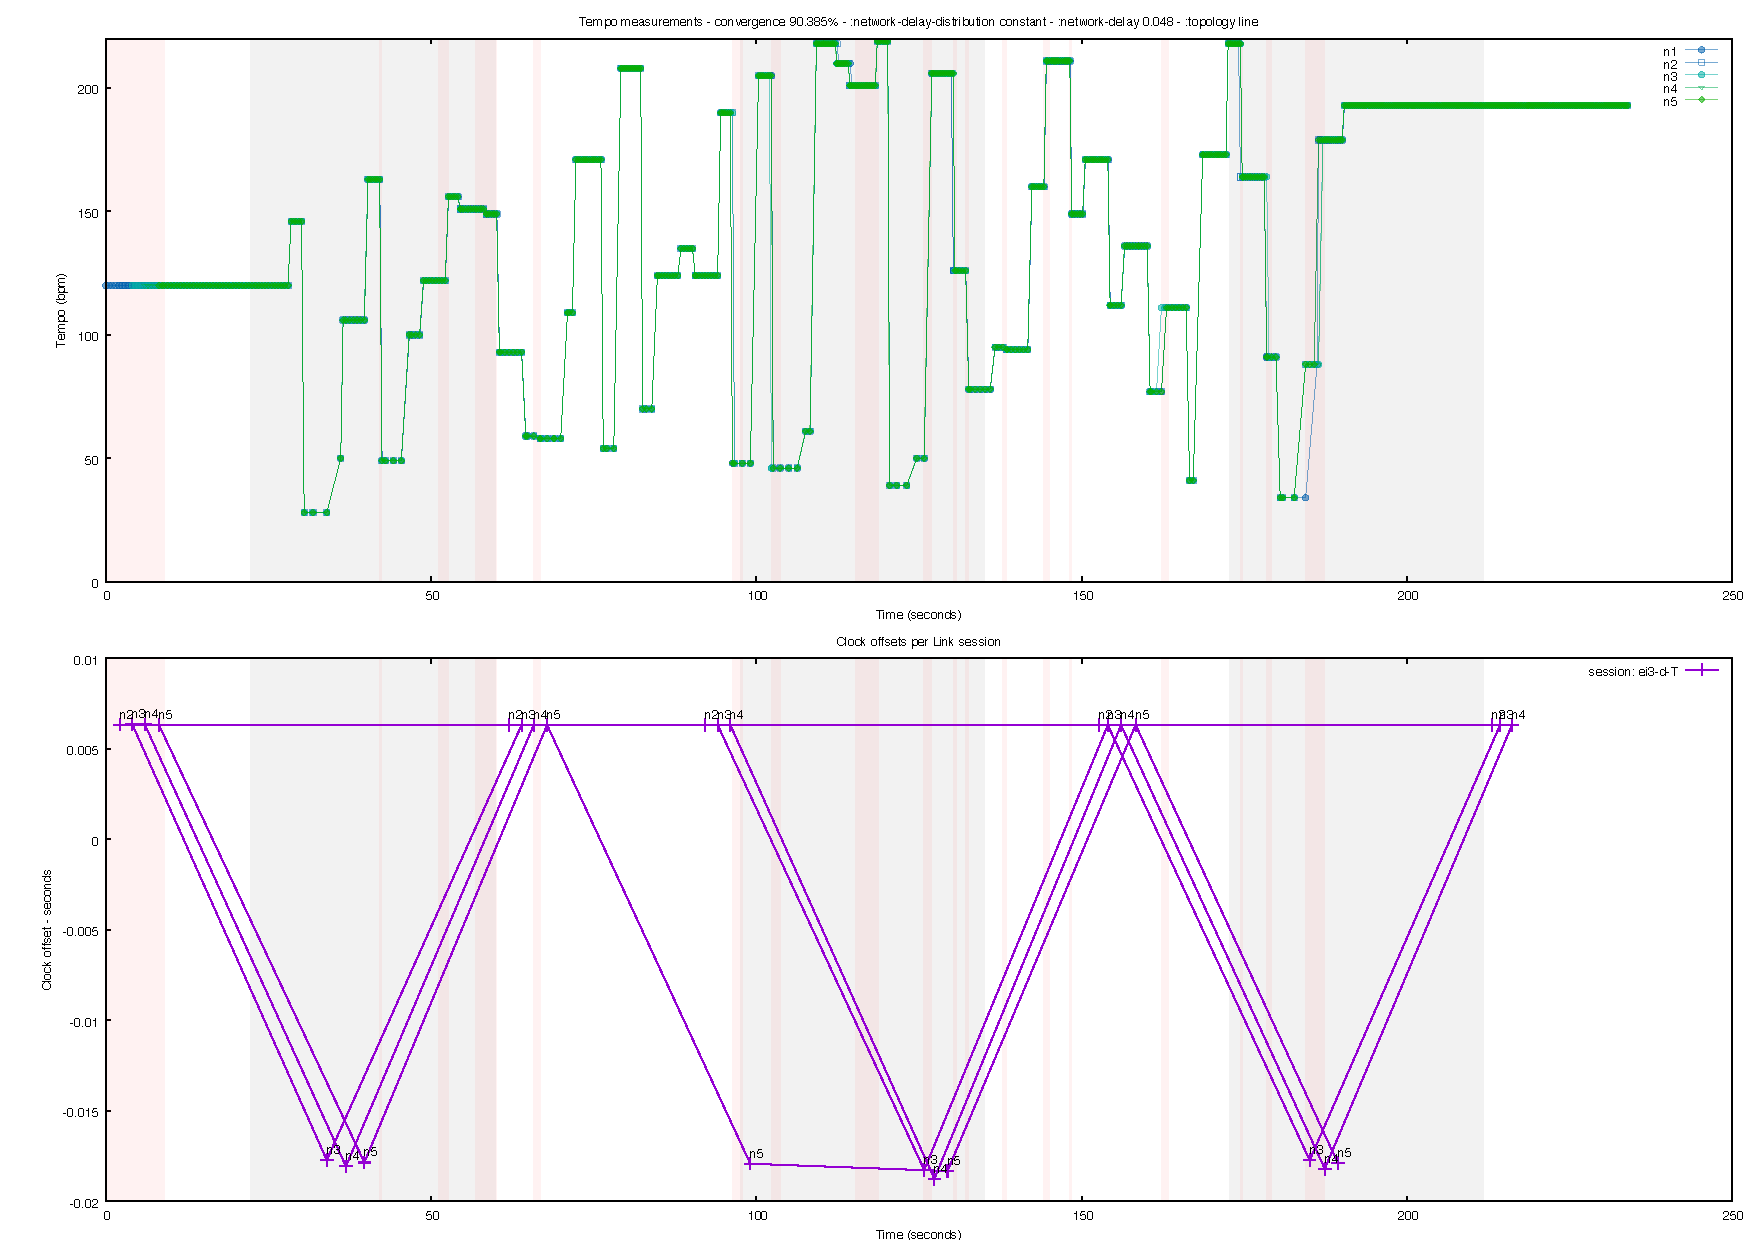
\includepdf[pages=-,angle=-90]{figures-for-publication/tempo_measurements_convergence_90_385_network_delay_distribution_constant_network_delay_0_048_topology_line/plot.pdf}
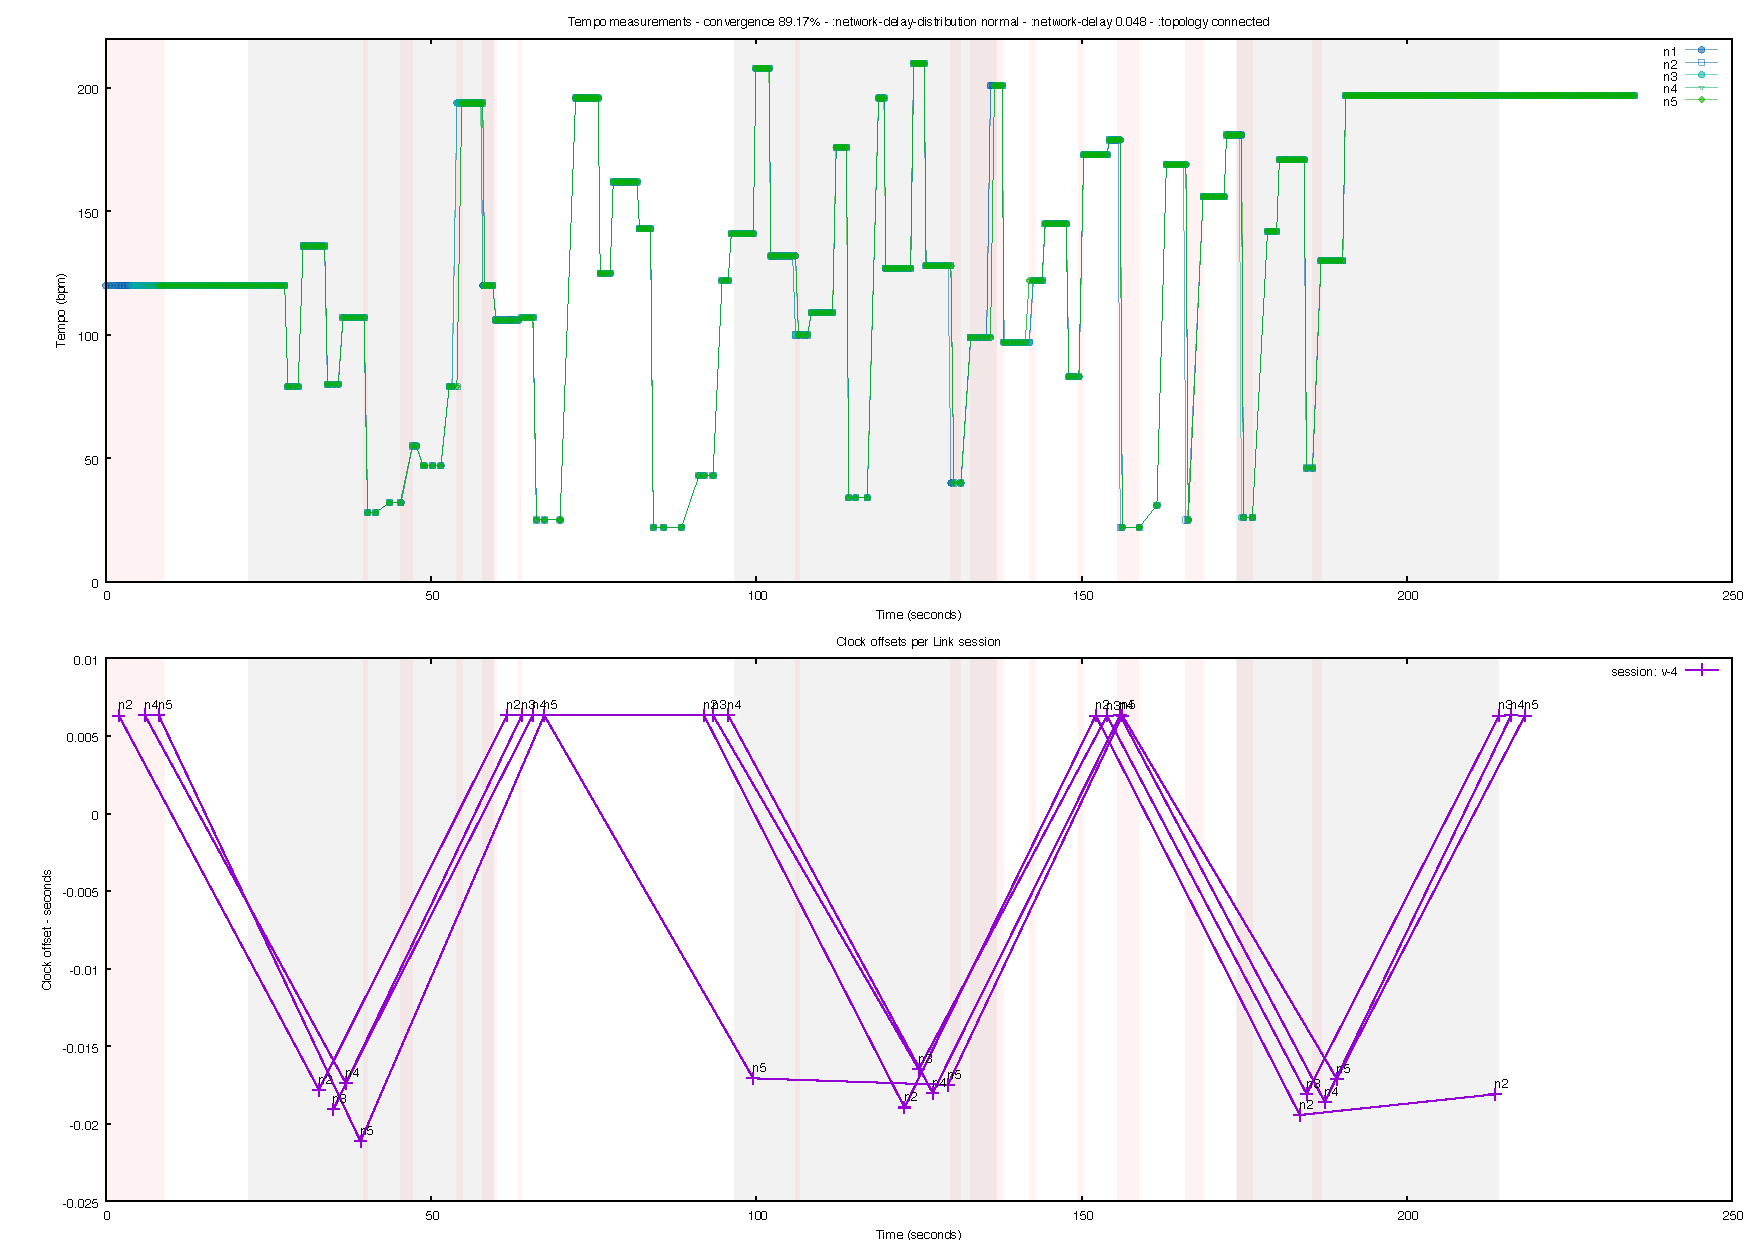
\includepdf[pages=-,angle=-90]{figures-for-publication/tempo_measurements_convergence_89_17_network_delay_distribution_normal_network_delay_0_048_topology_connected/plot.pdf}
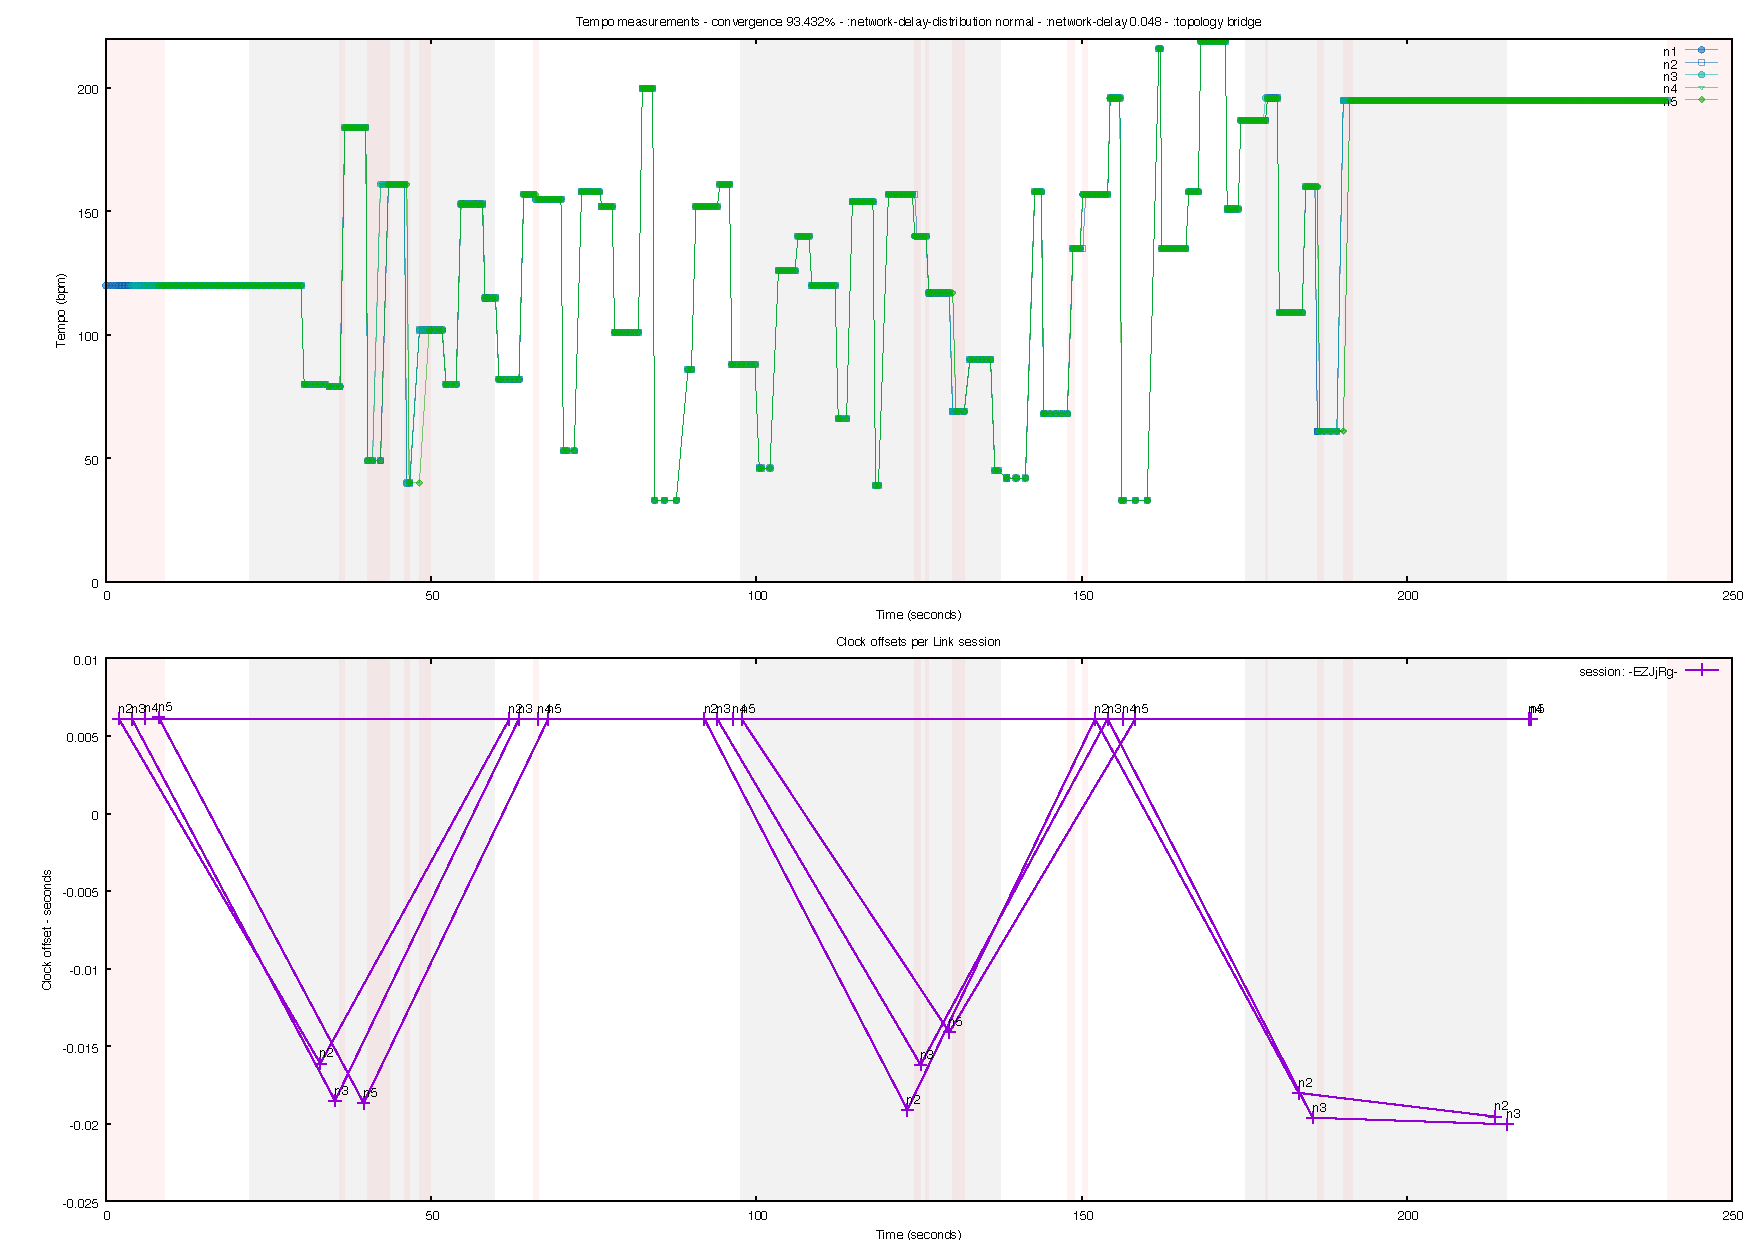
\includepdf[pages=-,angle=-90]{figures-for-publication/tempo_measurements_convergence_93_432_network_delay_distribution_normal_network_delay_0_048_topology_bridge/plot.pdf}
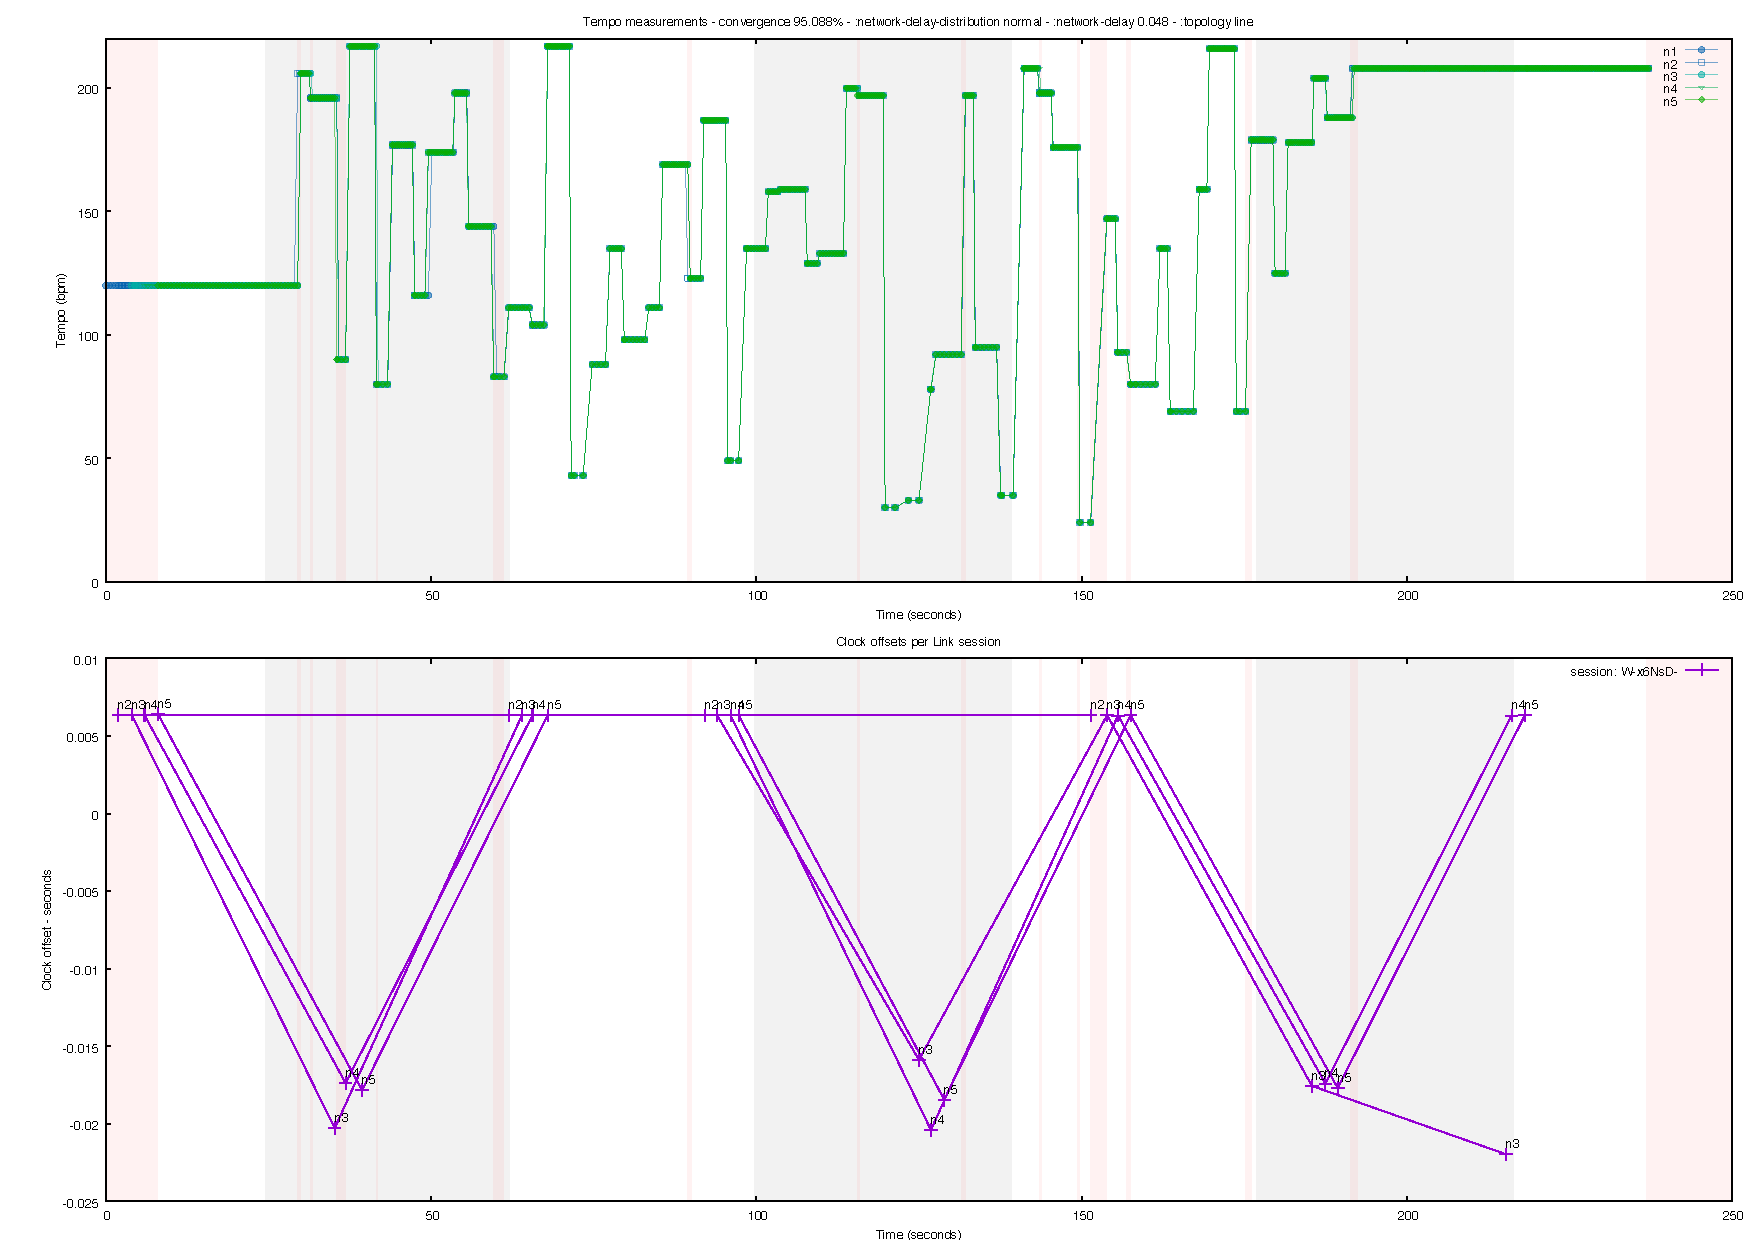
\includepdf[pages=-,angle=-90]{figures-for-publication/tempo_measurements_convergence_95_088_network_delay_distribution_normal_network_delay_0_048_topology_line/plot.pdf}
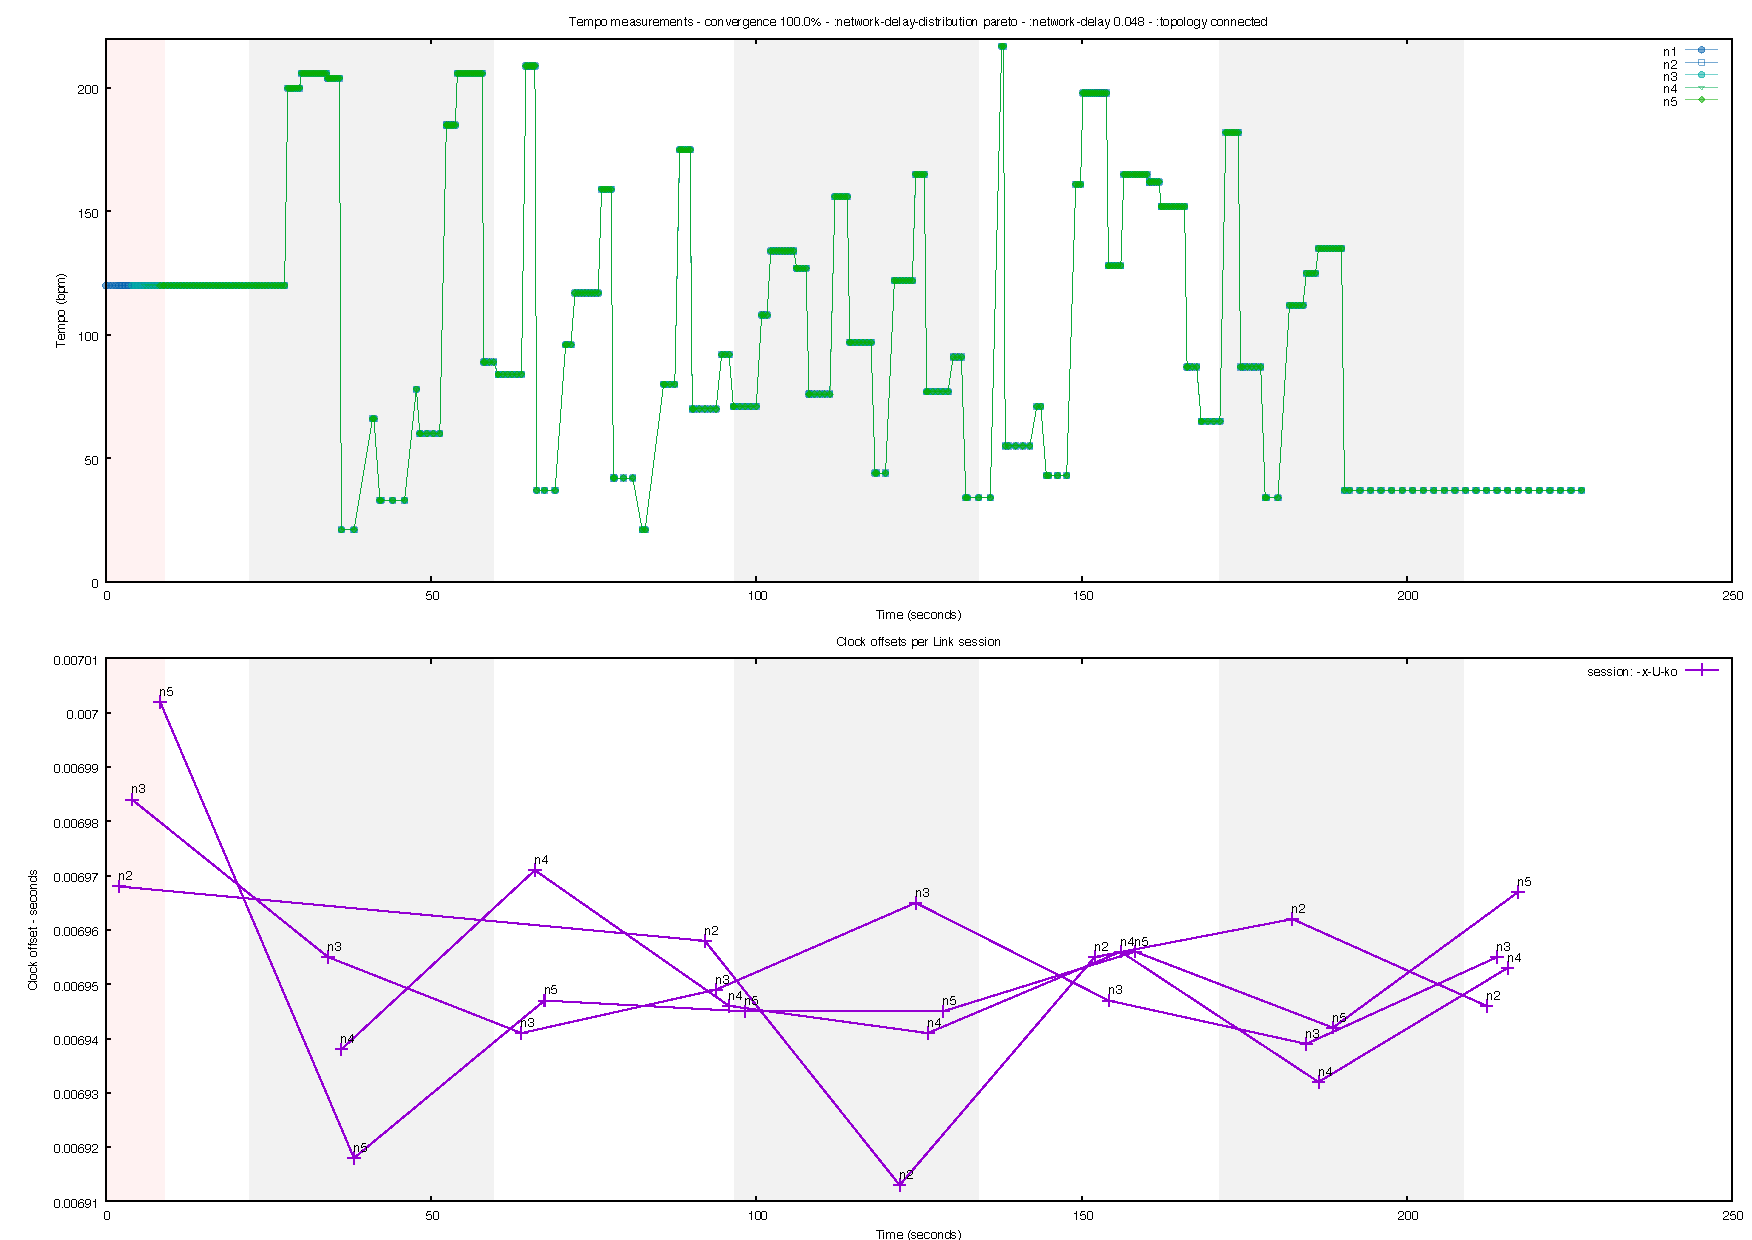
\includepdf[pages=-,angle=-90]{figures-for-publication/tempo_measurements_convergence_100_0_network_delay_distribution_pareto_network_delay_0_048_topology_connected/plot.pdf}
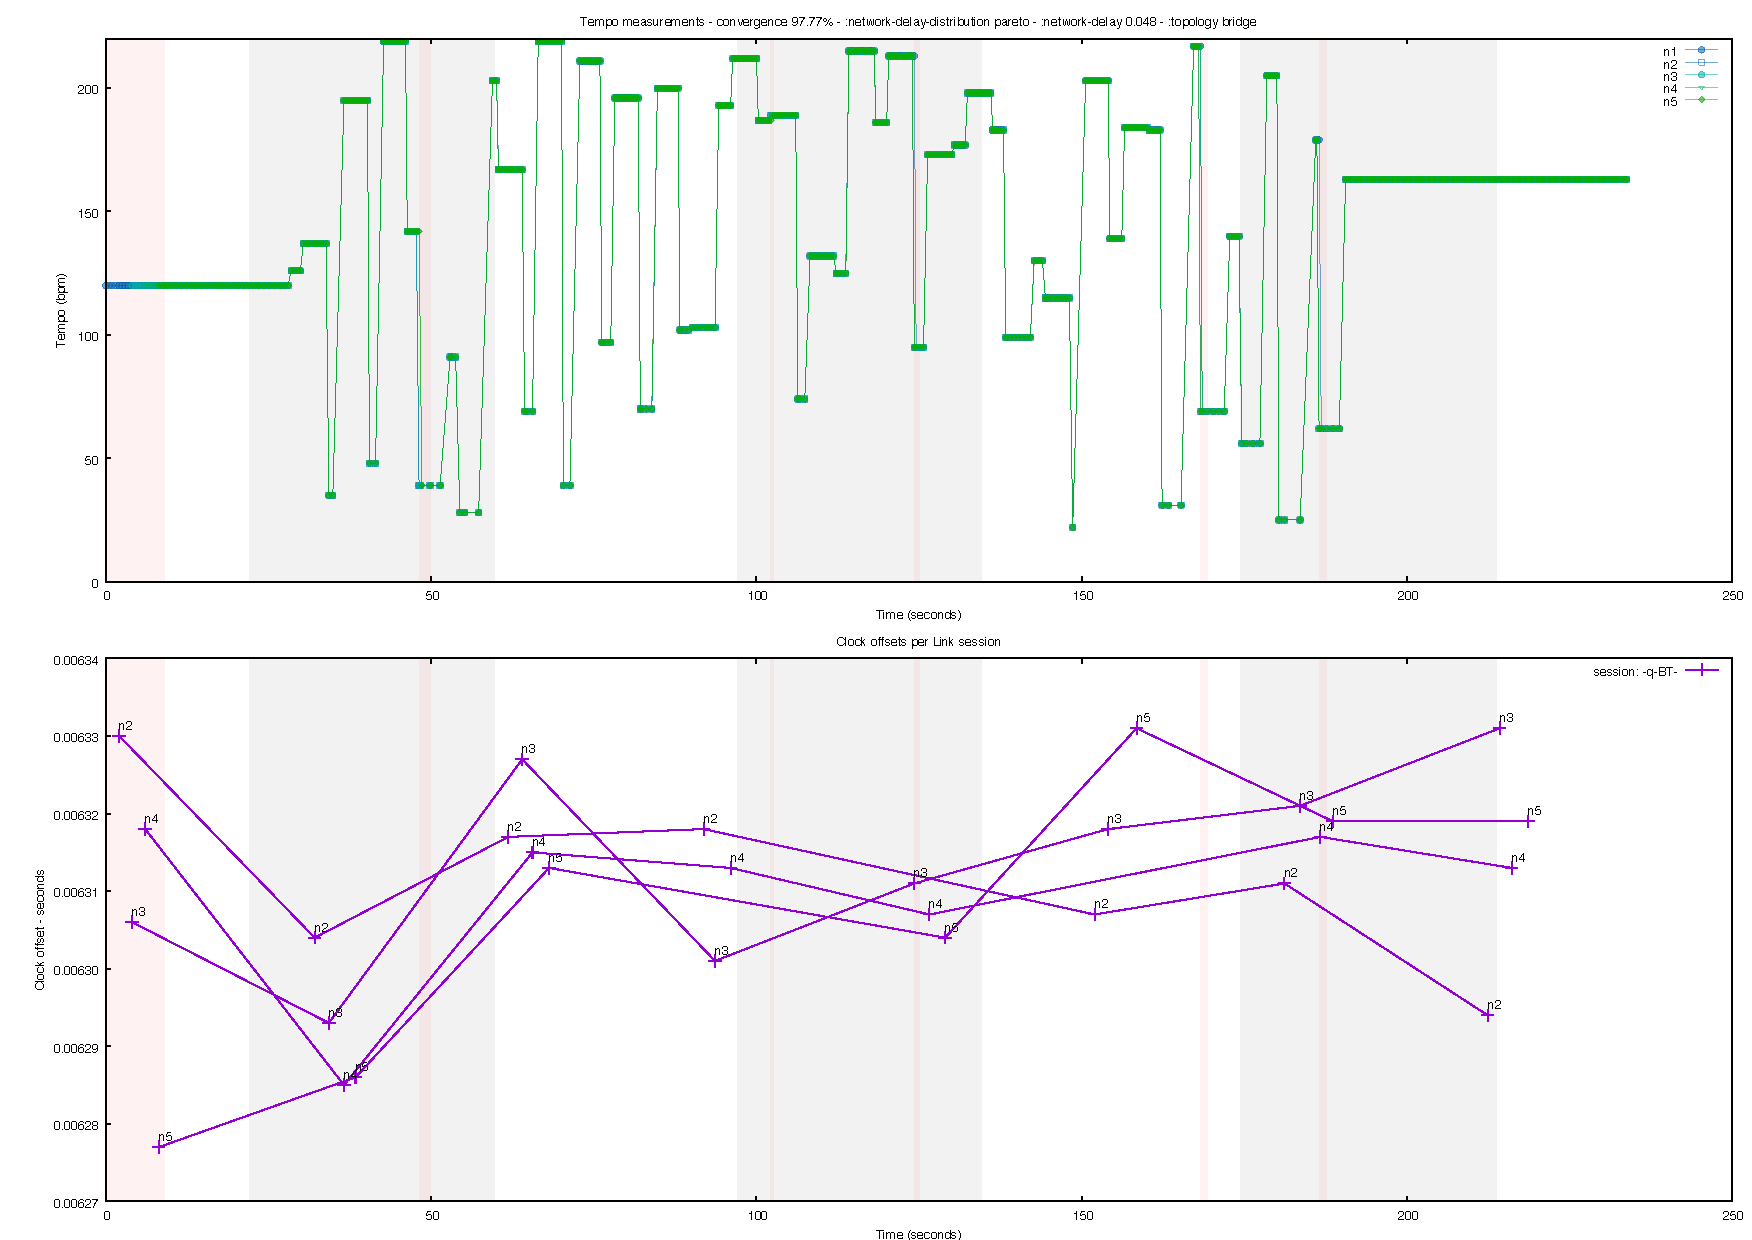
\includepdf[pages=-,angle=-90]{figures-for-publication/tempo_measurements_convergence_97_77_network_delay_distribution_pareto_network_delay_0_048_topology_bridge/plot.pdf}
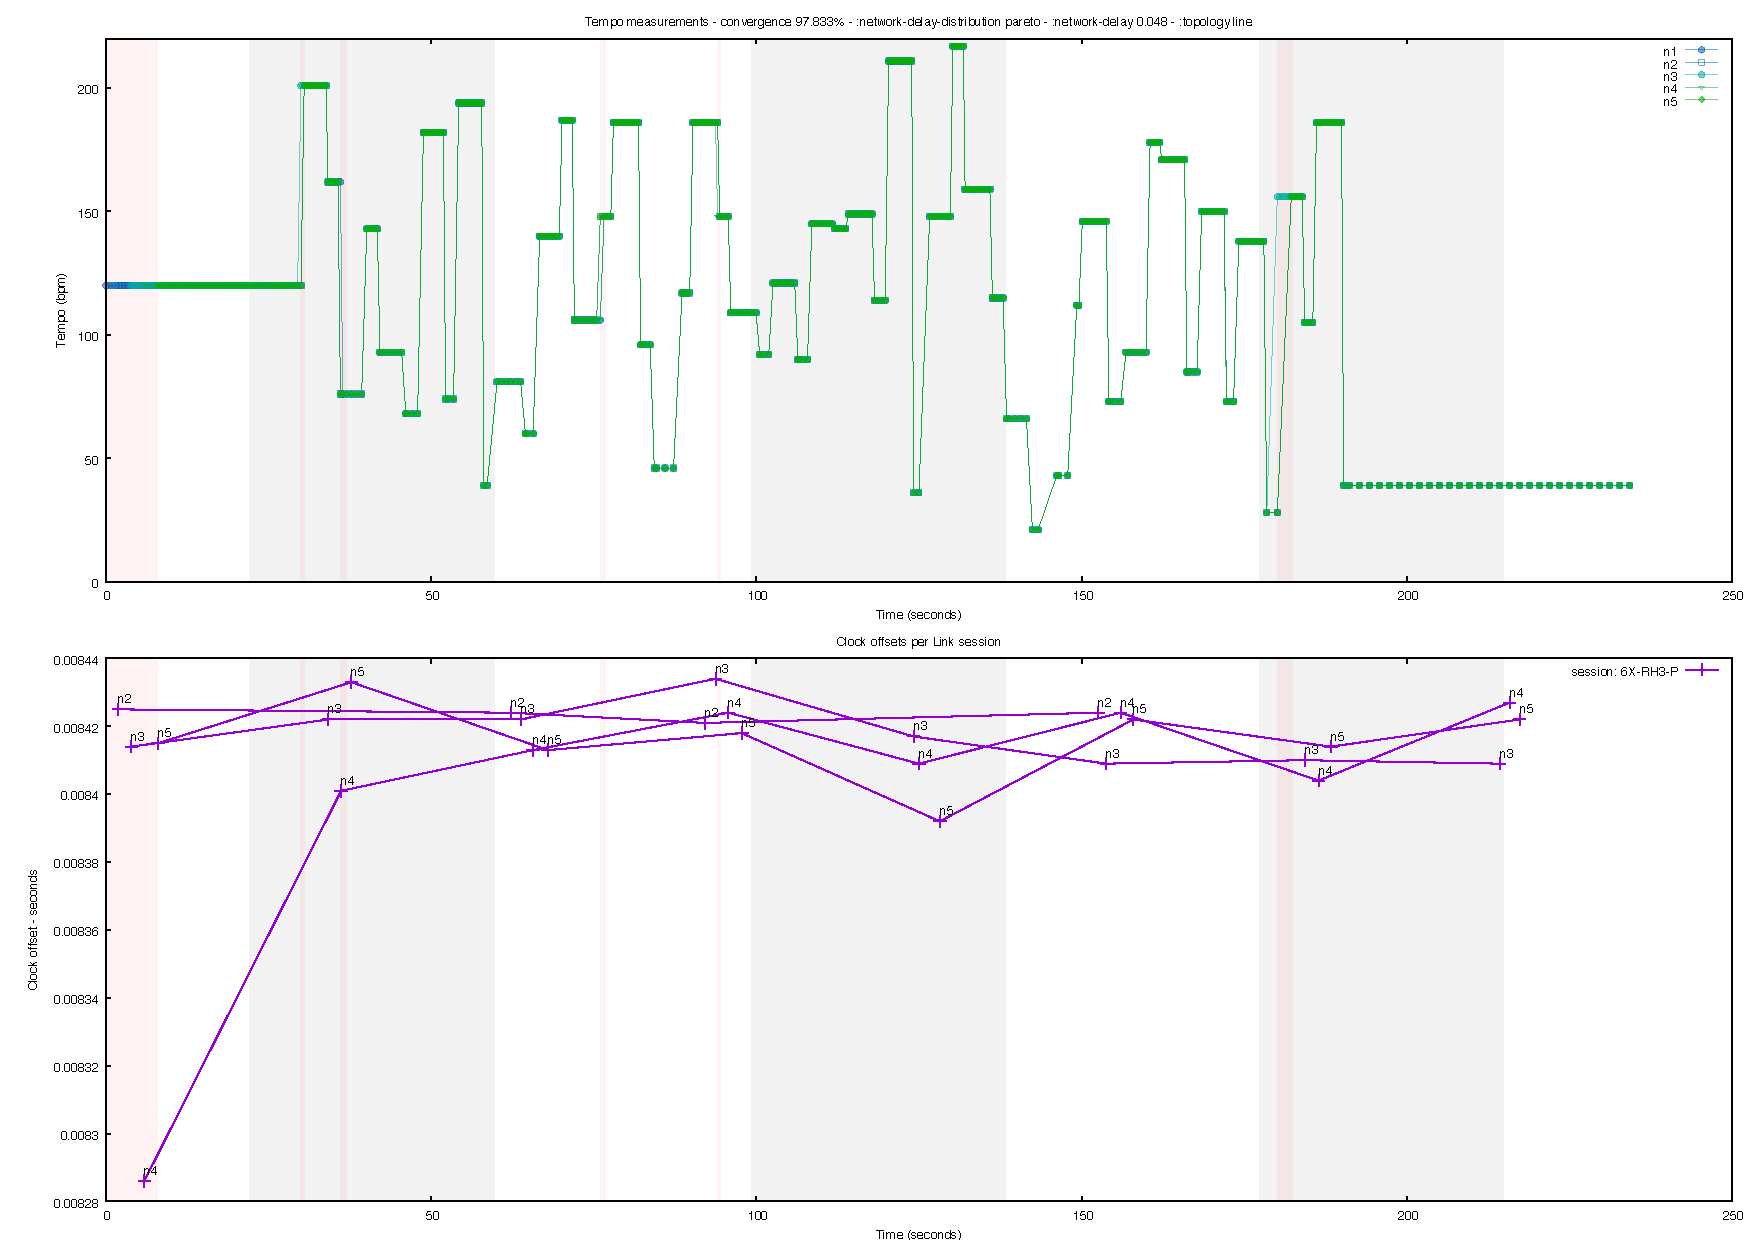
\includepdf[pages=-,angle=-90]{figures-for-publication/tempo_measurements_convergence_97_833_network_delay_distribution_pareto_network_delay_0_048_topology_line/plot.pdf}

% 500ms delays
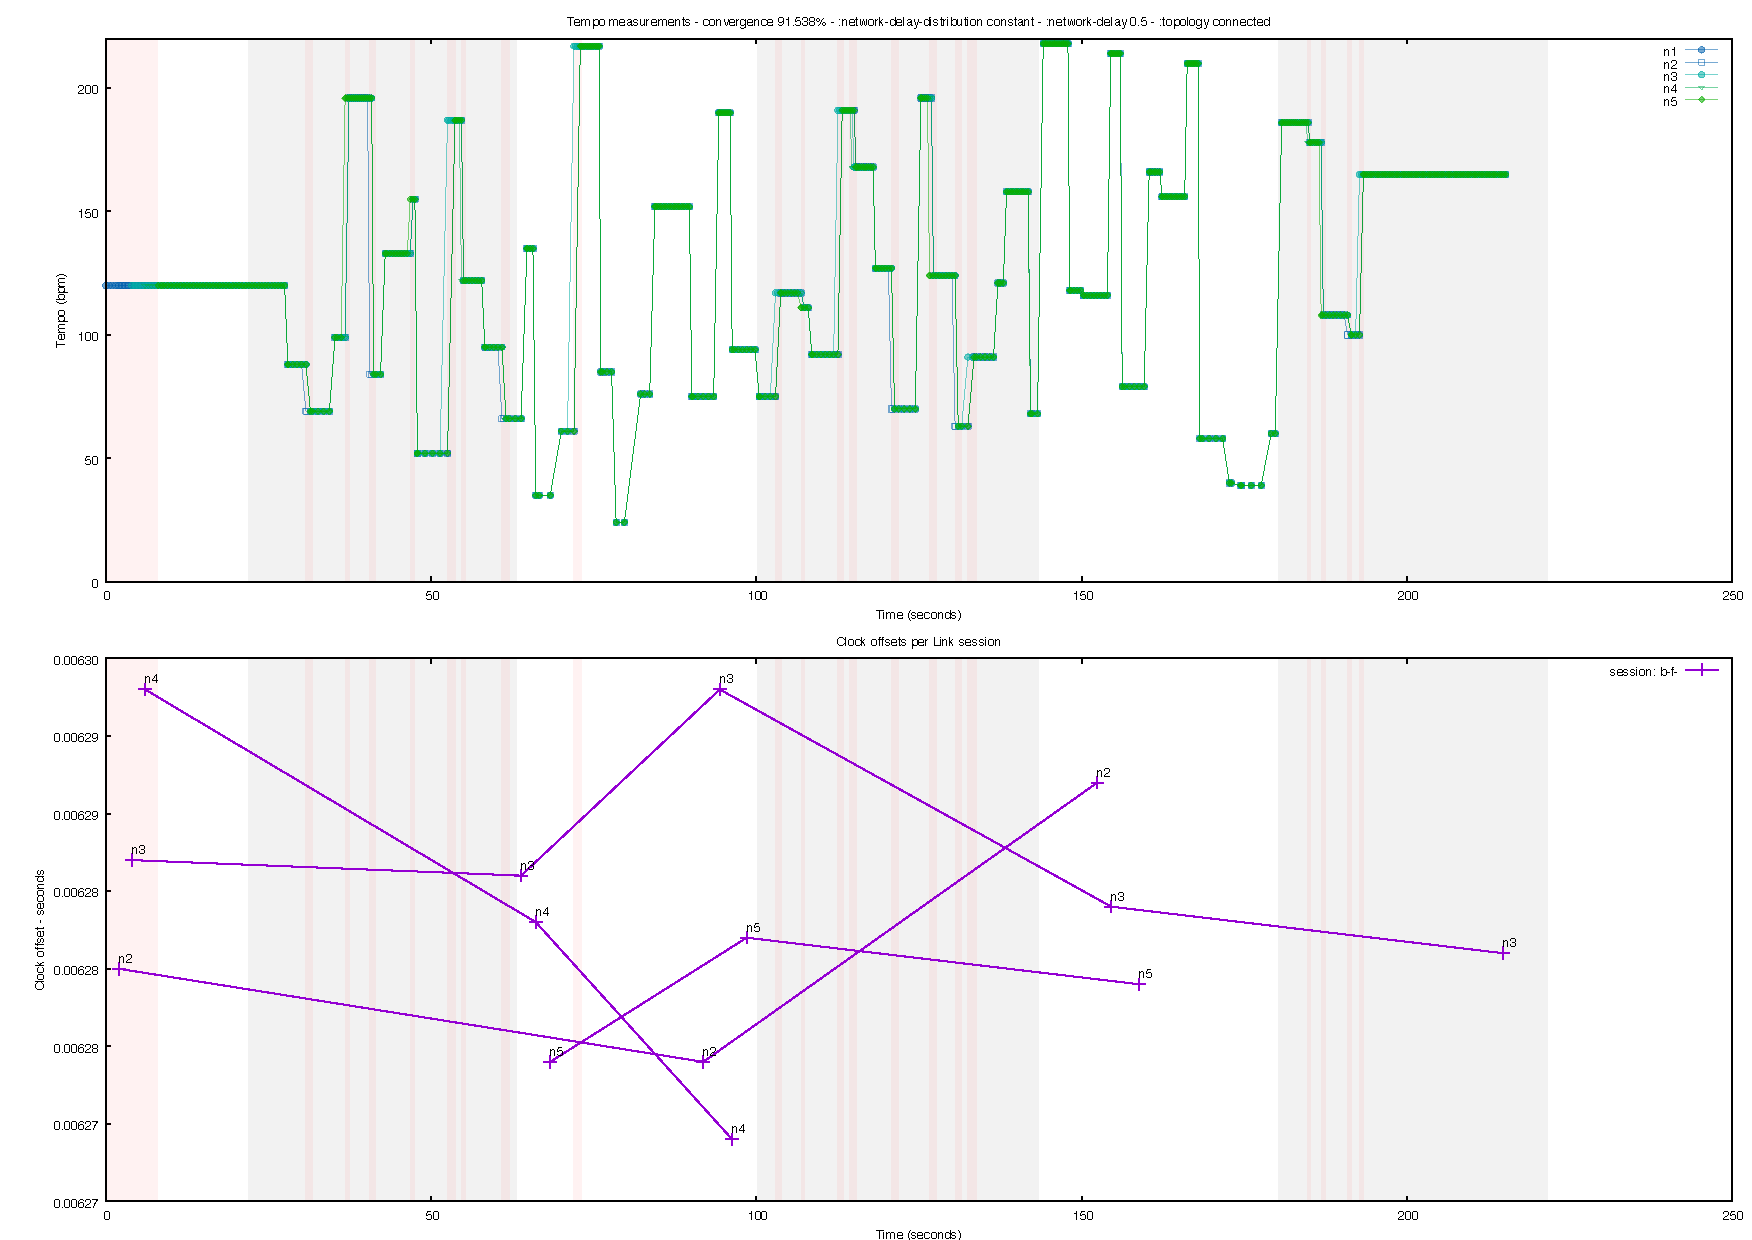
\includepdf[pages=-,angle=-90]{figures-for-publication/tempo_measurements_convergence_91_538_network_delay_distribution_constant_network_delay_0_5_topology_connected/plot.pdf}
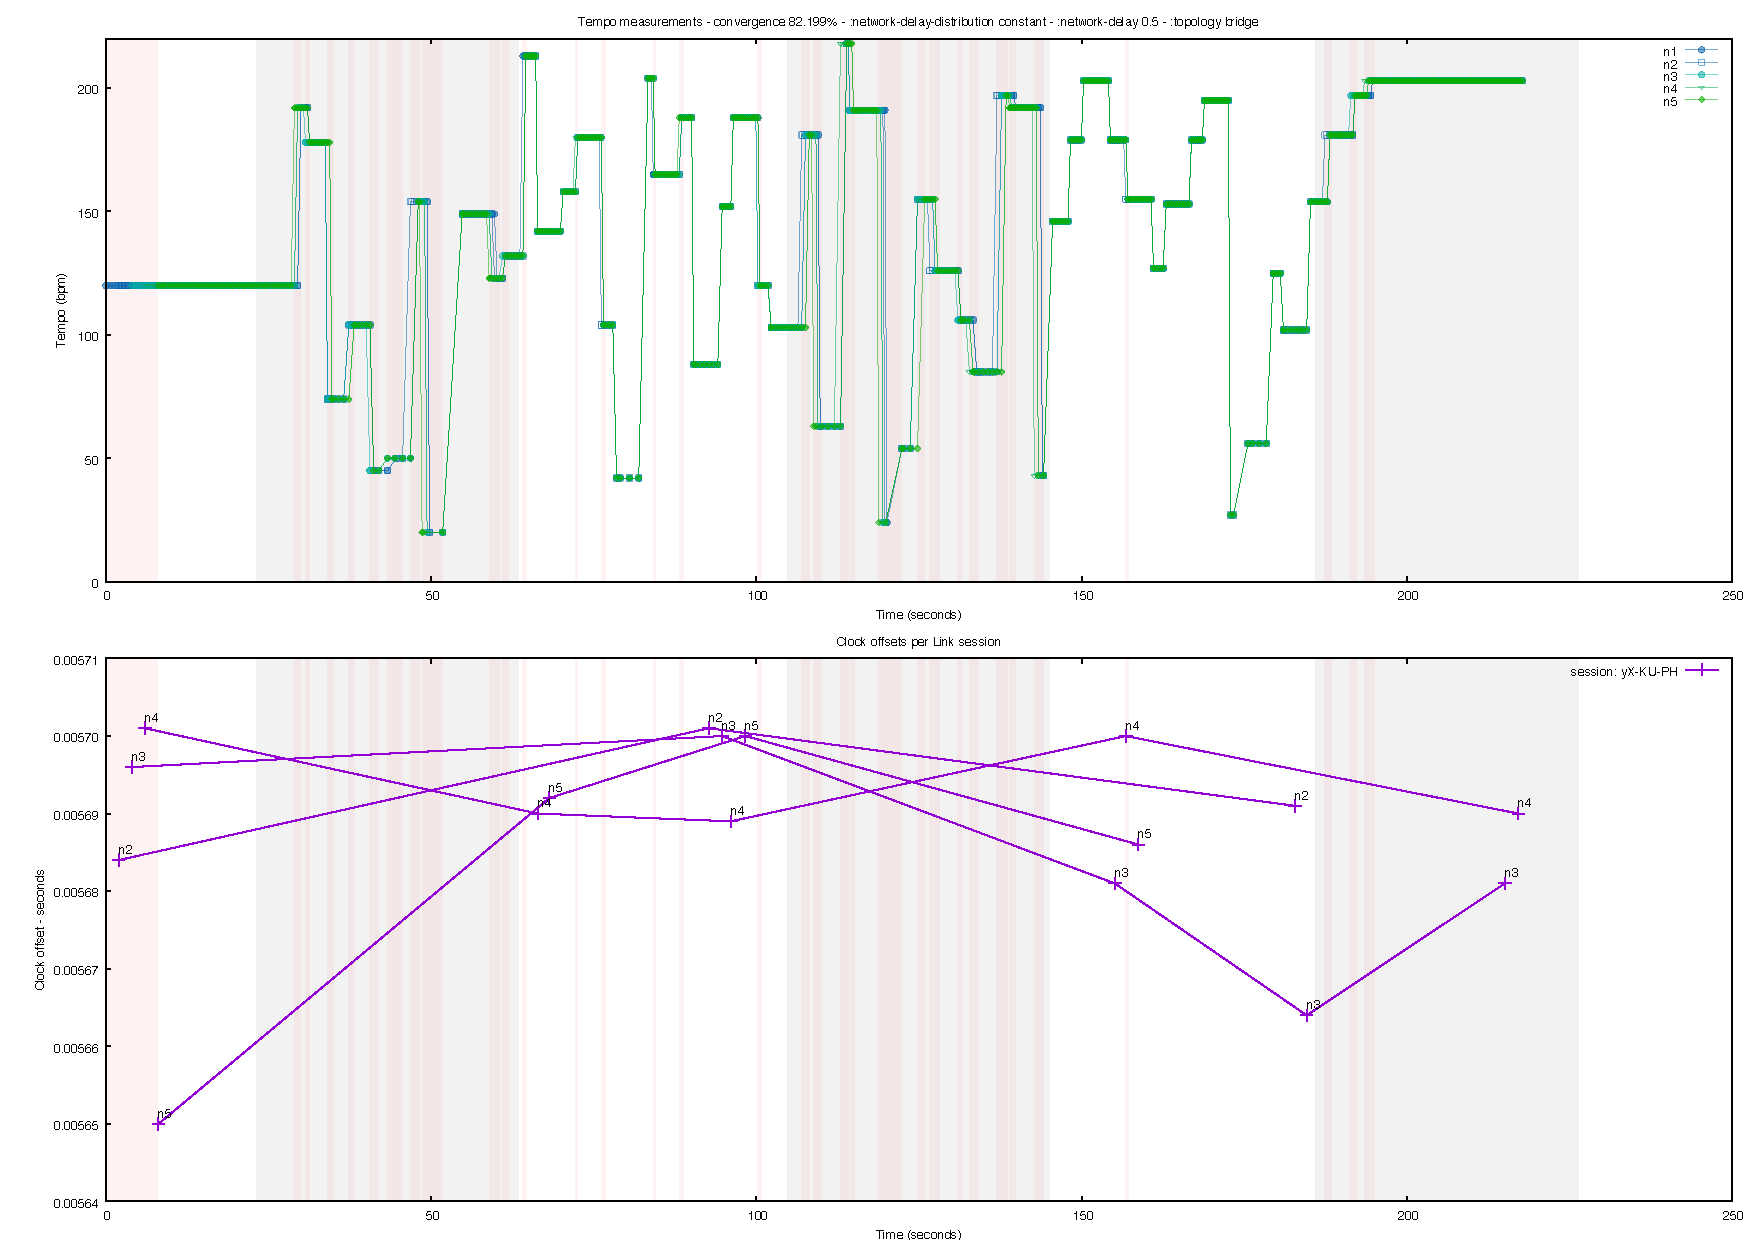
\includepdf[pages=-,angle=-90]{figures-for-publication/tempo_measurements_convergence_82_199_network_delay_distribution_constant_network_delay_0_5_topology_bridge/plot.pdf}
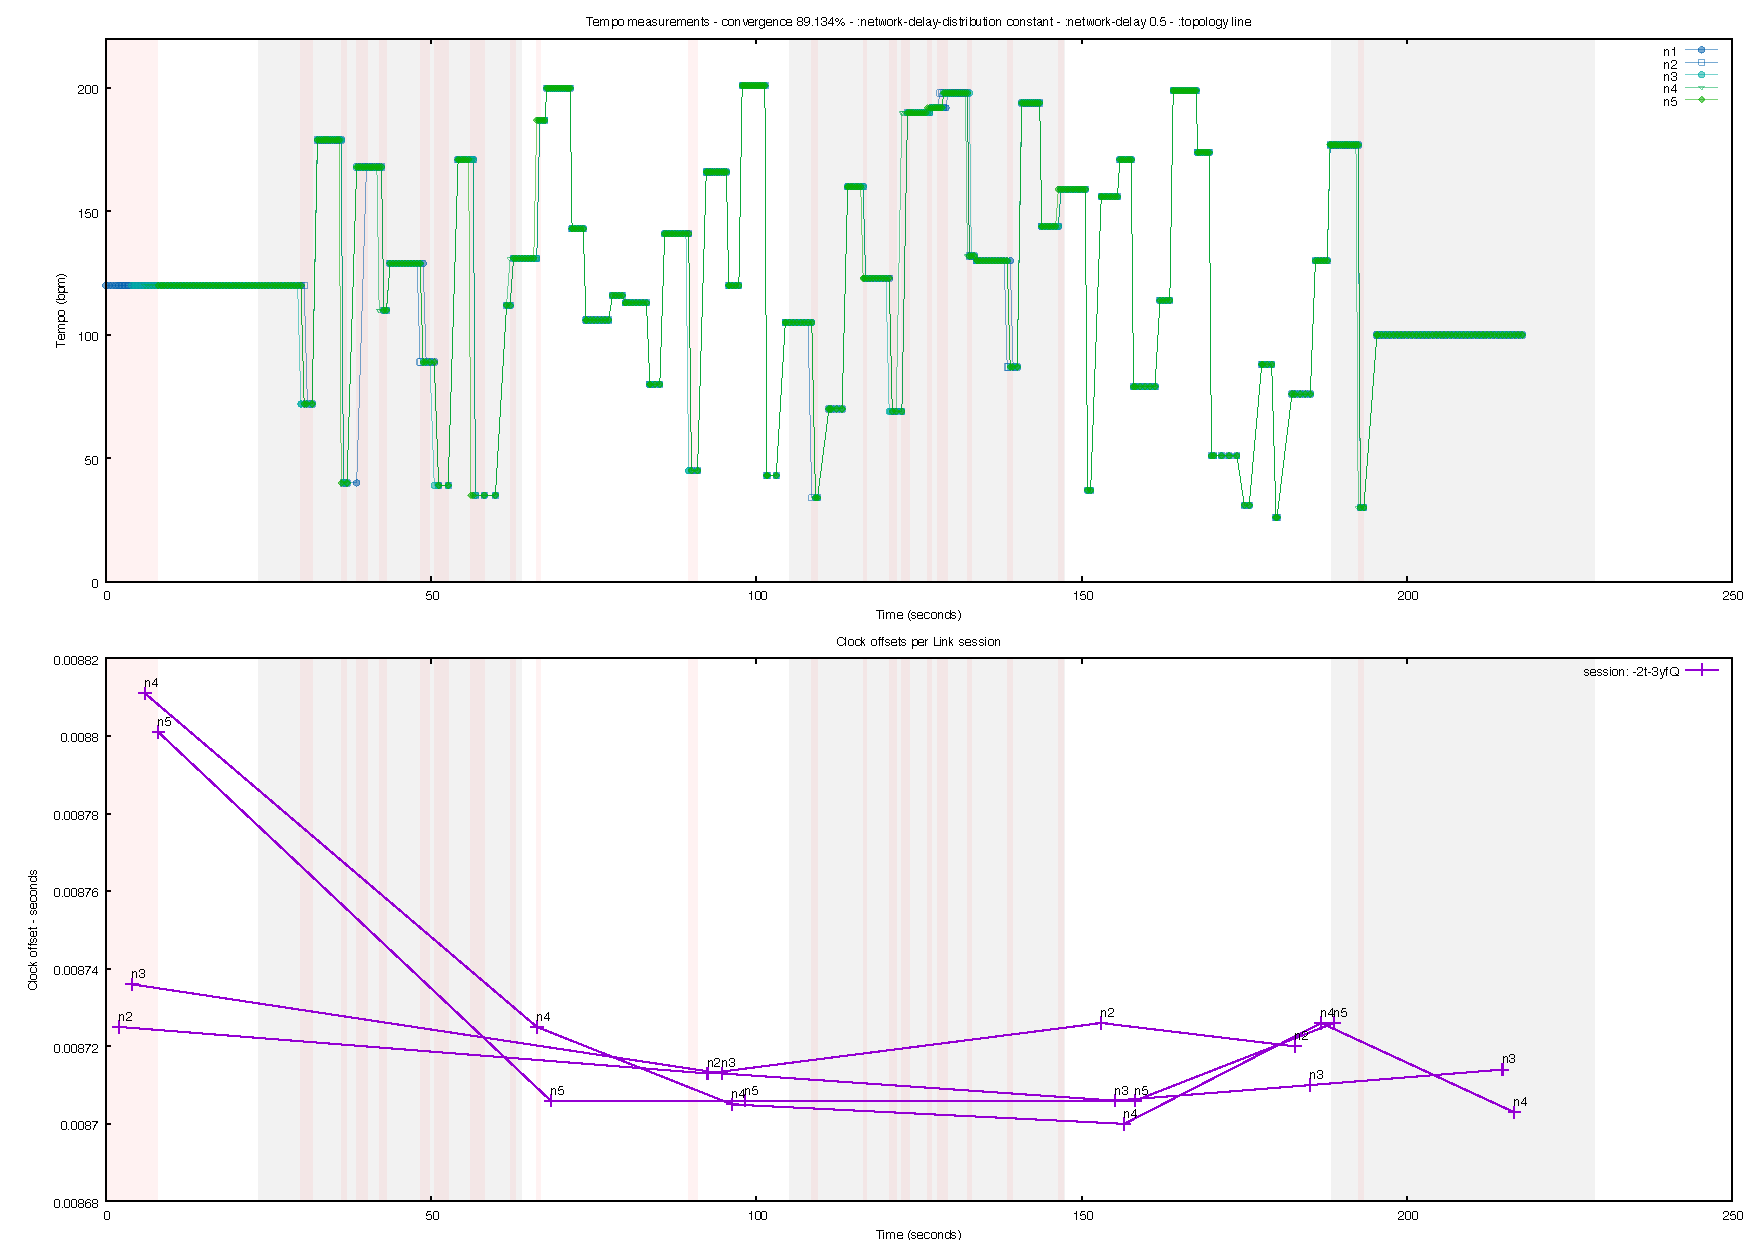
\includepdf[pages=-,angle=-90]{figures-for-publication/tempo_measurements_convergence_89_134_network_delay_distribution_constant_network_delay_0_5_topology_line/plot.pdf}
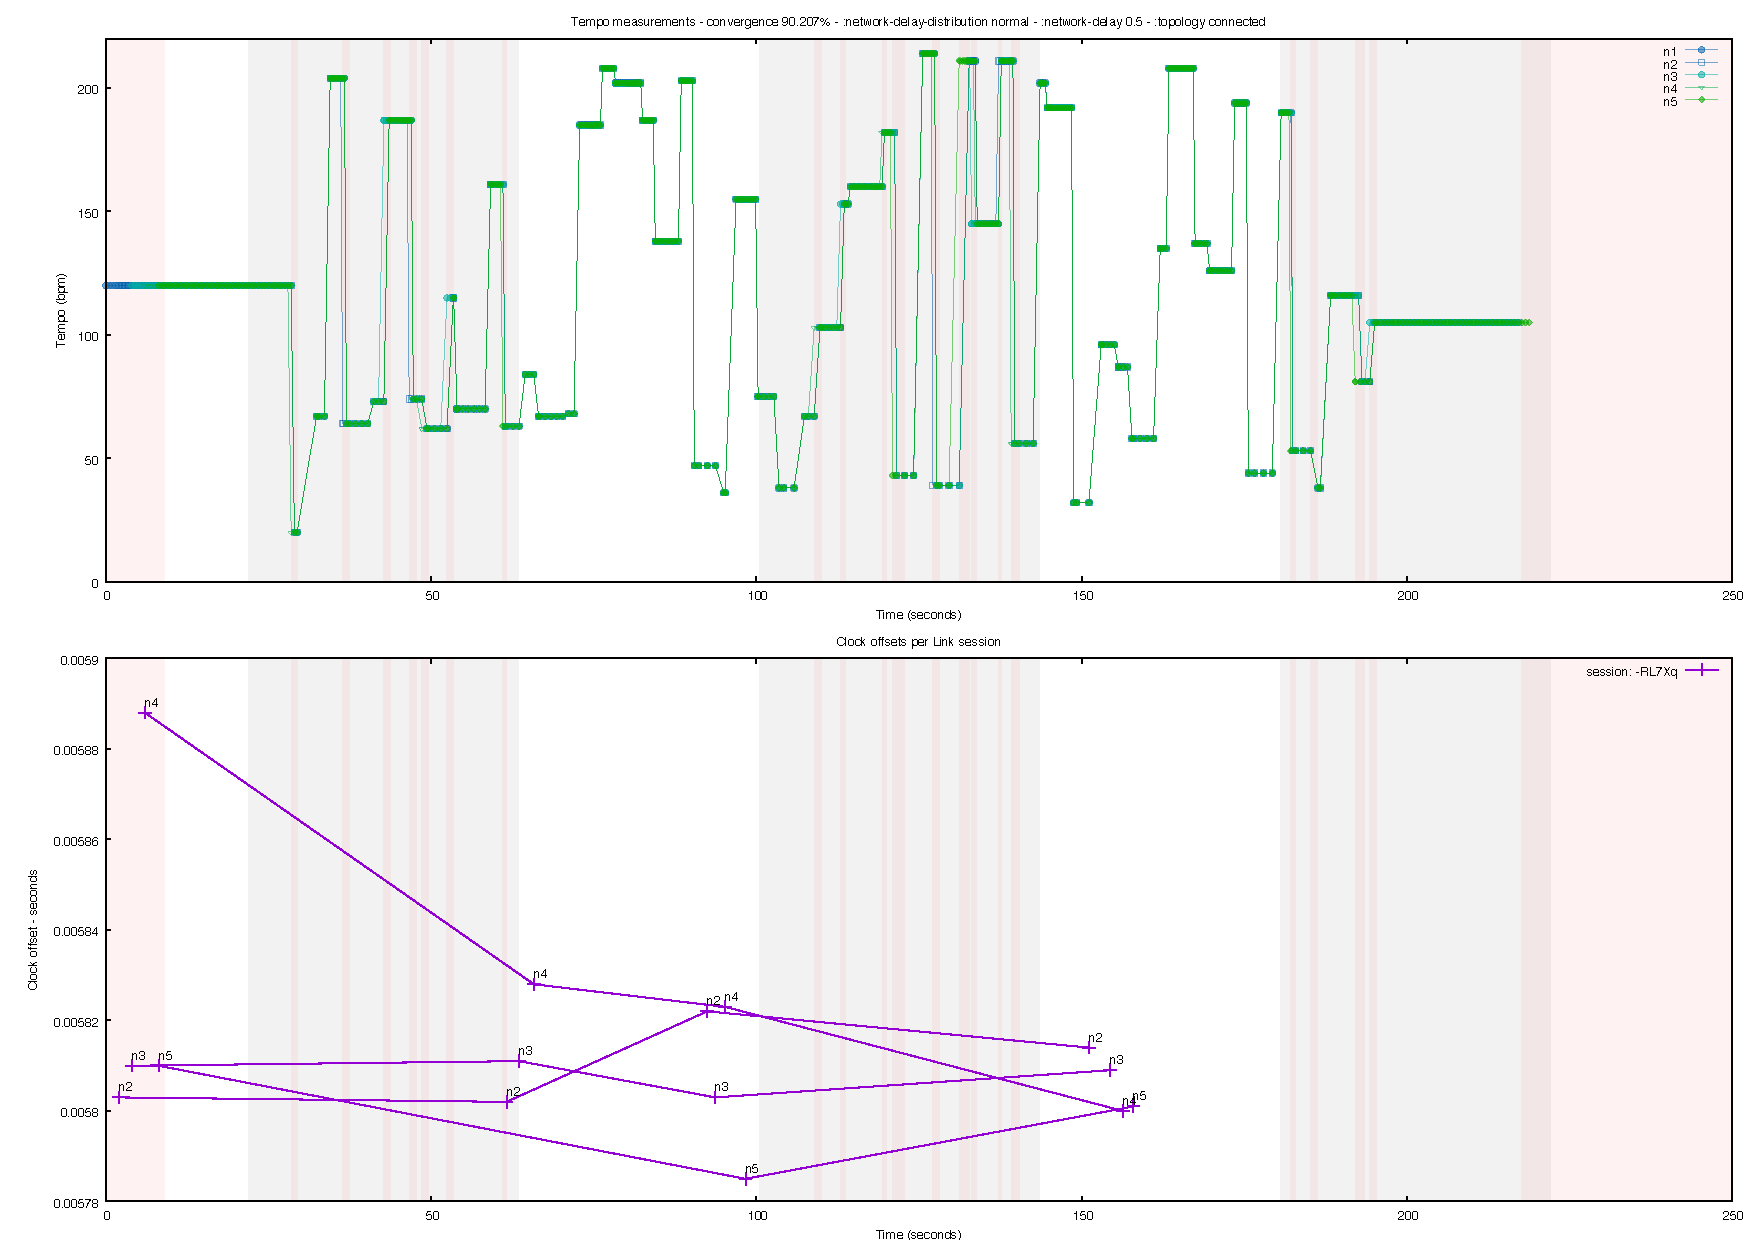
\includepdf[pages=-,angle=-90]{figures-for-publication/tempo_measurements_convergence_90_207_network_delay_distribution_normal_network_delay_0_5_topology_connected/plot.pdf}
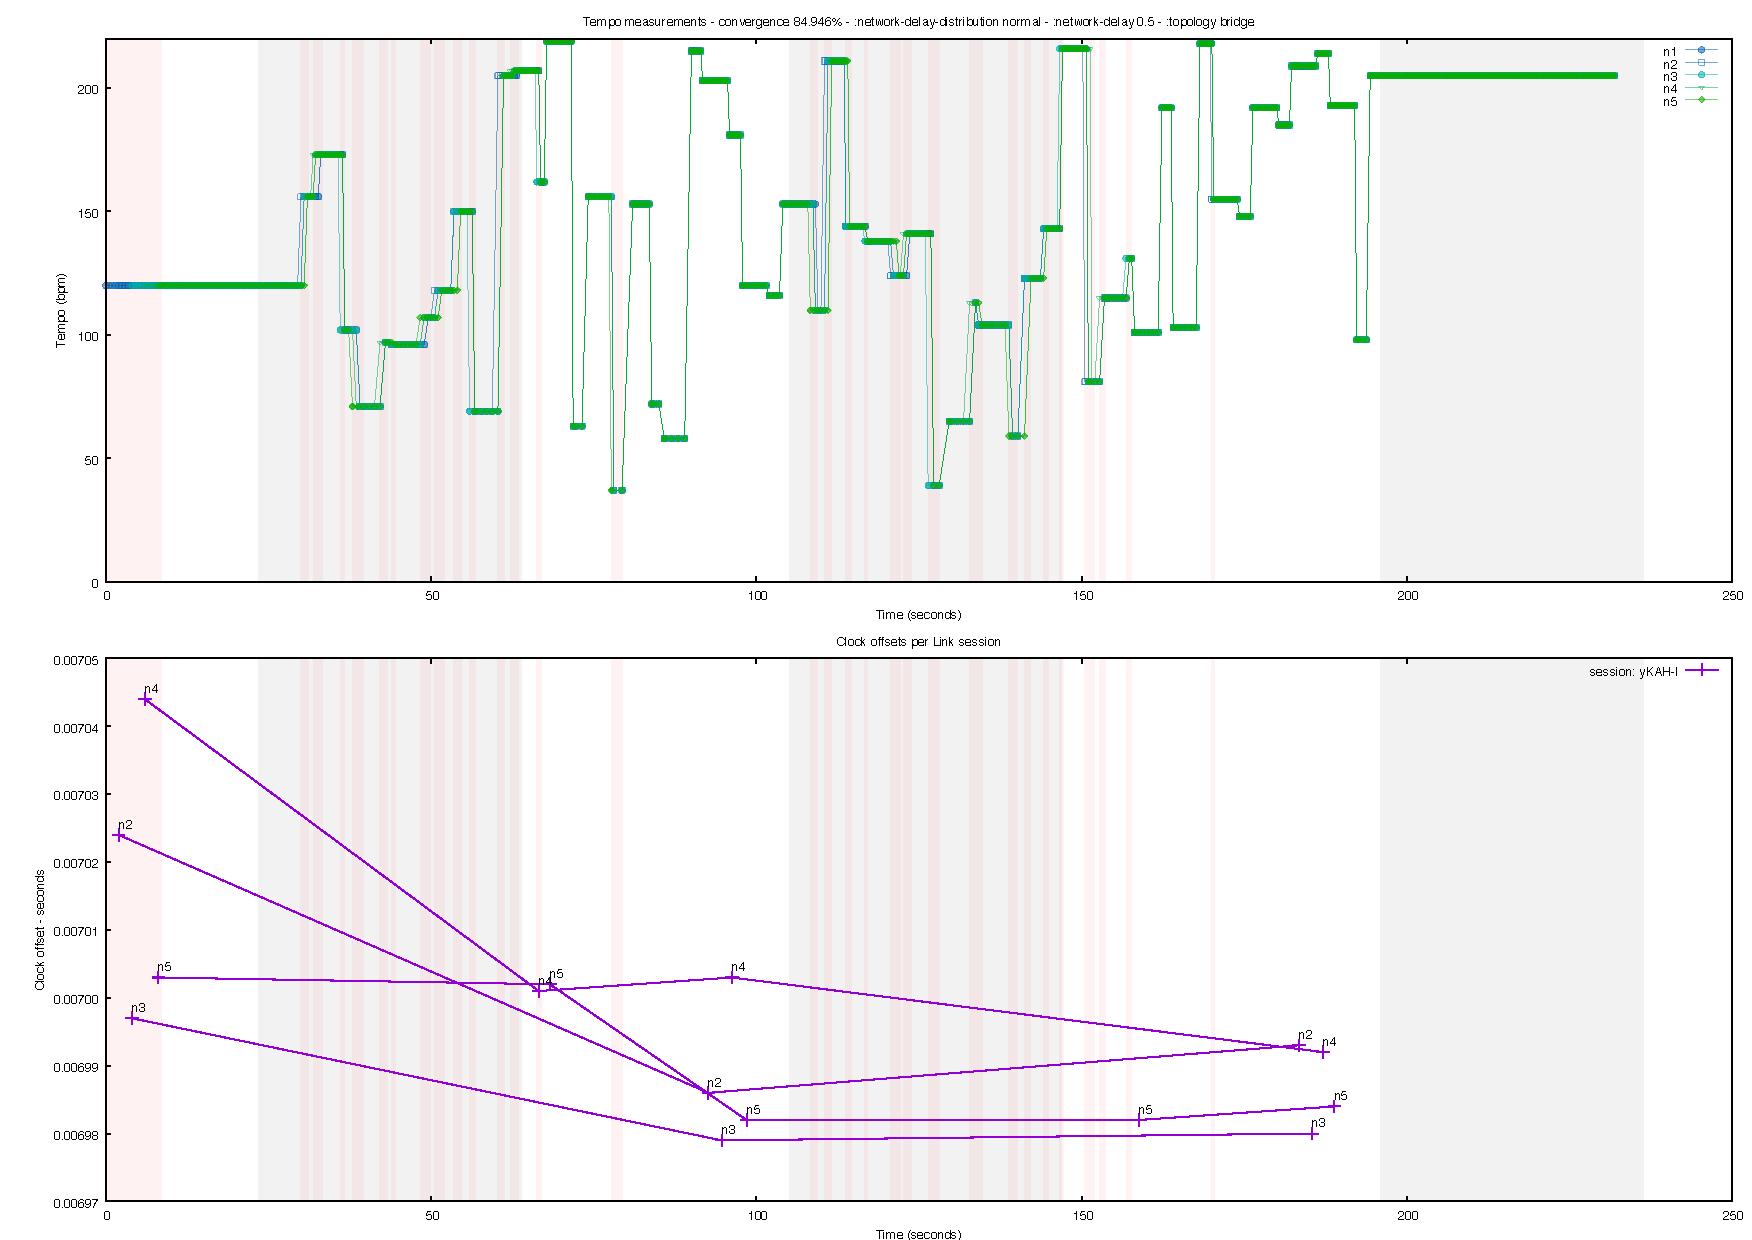
\includepdf[pages=-,angle=-90]{figures-for-publication/tempo_measurements_convergence_84_946_network_delay_distribution_normal_network_delay_0_5_topology_bridge/plot.pdf}
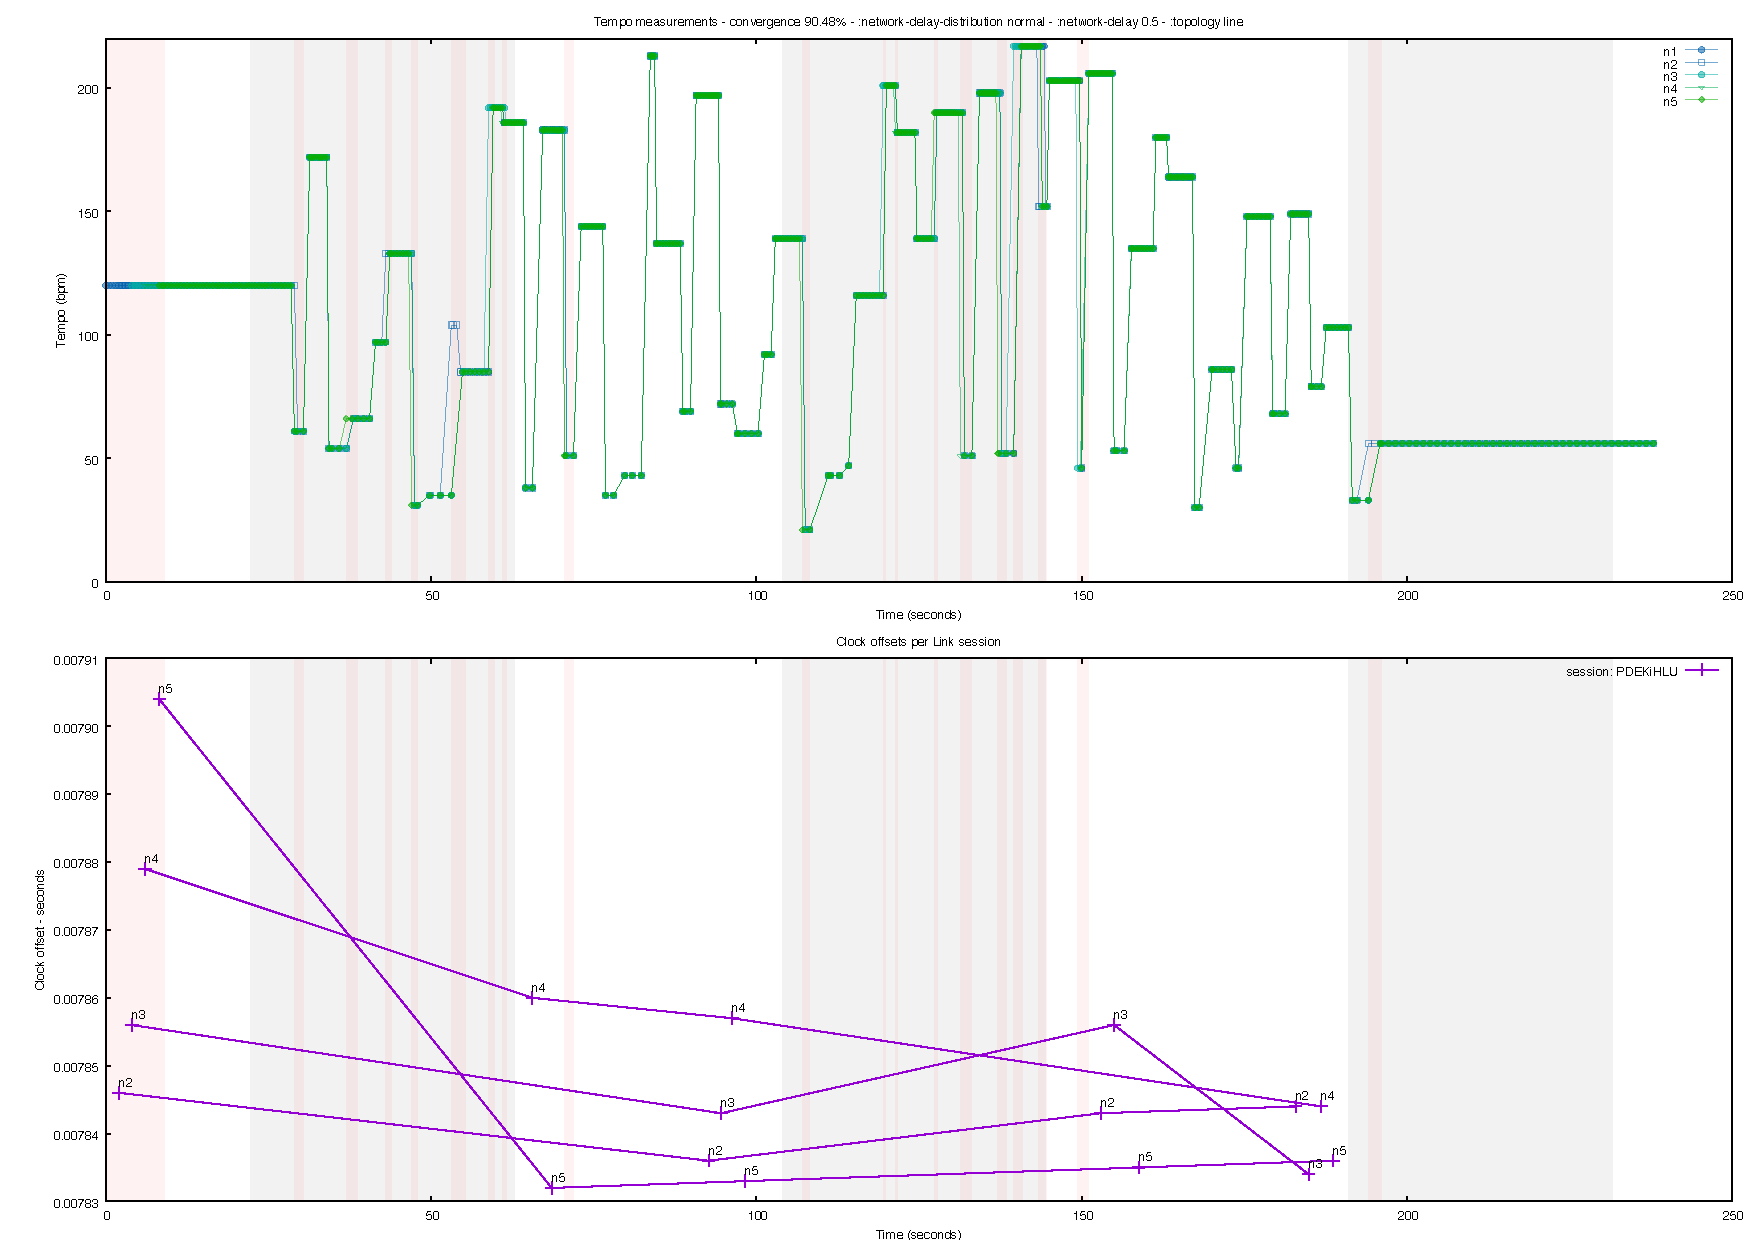
\includepdf[pages=-,angle=-90]{figures-for-publication/tempo_measurements_convergence_90_48_network_delay_distribution_normal_network_delay_0_5_topology_line/plot.pdf}
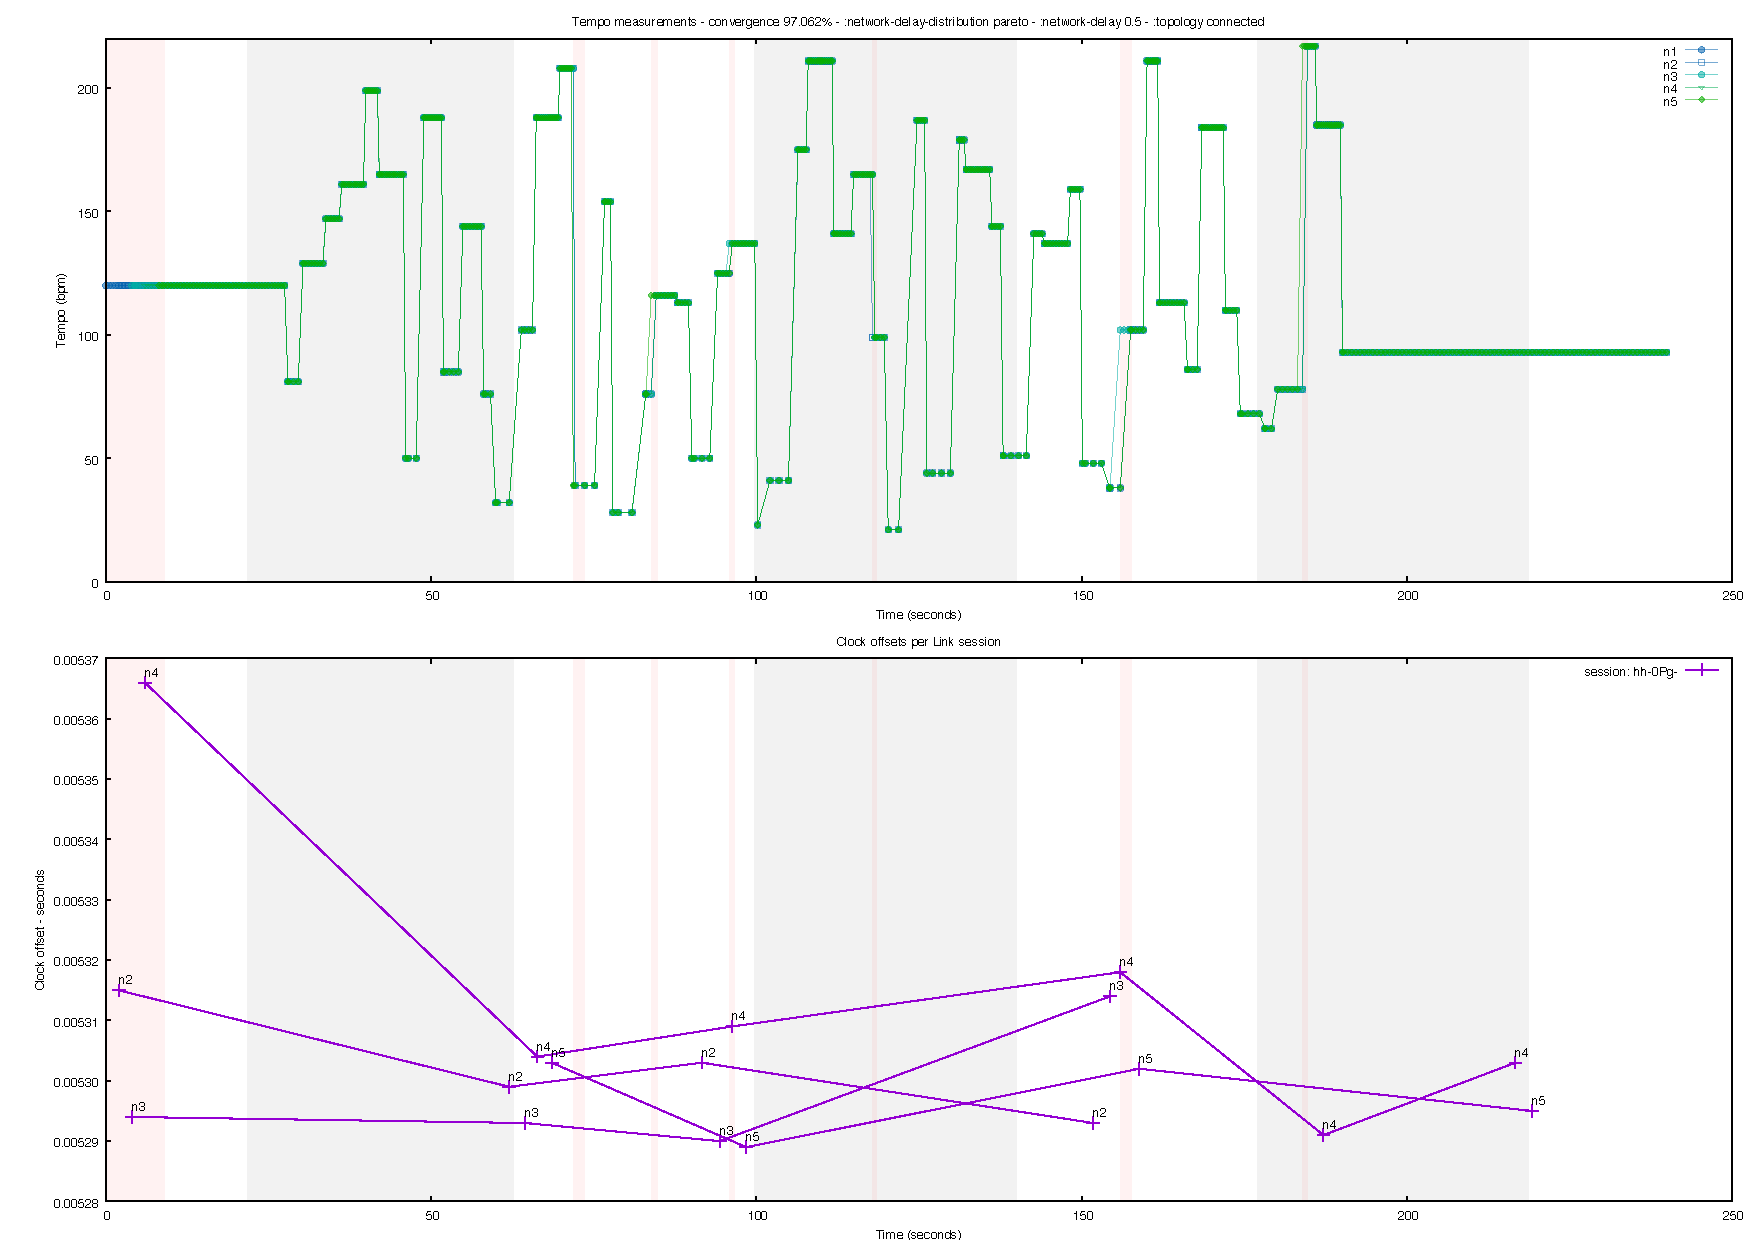
\includepdf[pages=-,angle=-90]{figures-for-publication/tempo_measurements_convergence_97_062_network_delay_distribution_pareto_network_delay_0_5_topology_connected/plot.pdf}
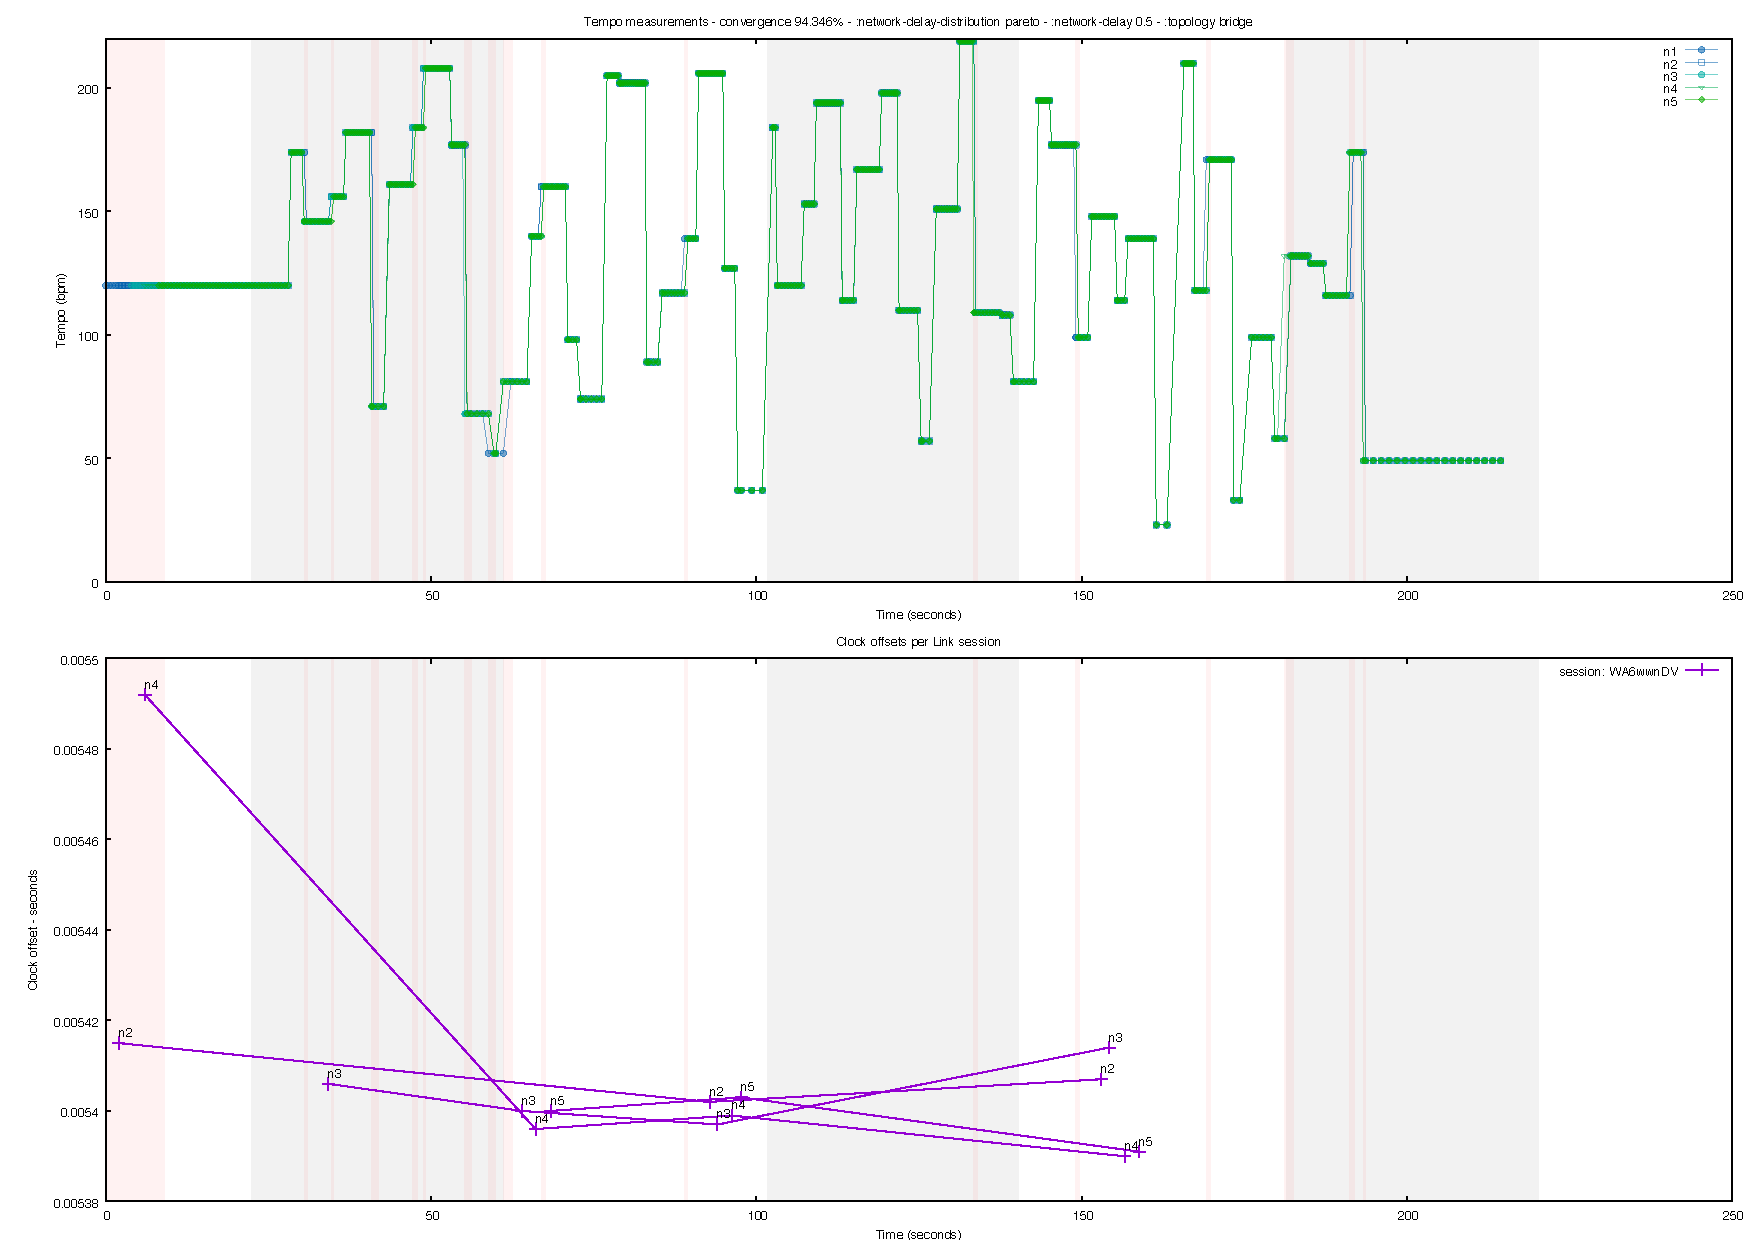
\includepdf[pages=-,angle=-90]{figures-for-publication/tempo_measurements_convergence_94_346_network_delay_distribution_pareto_network_delay_0_5_topology_bridge/plot.pdf}
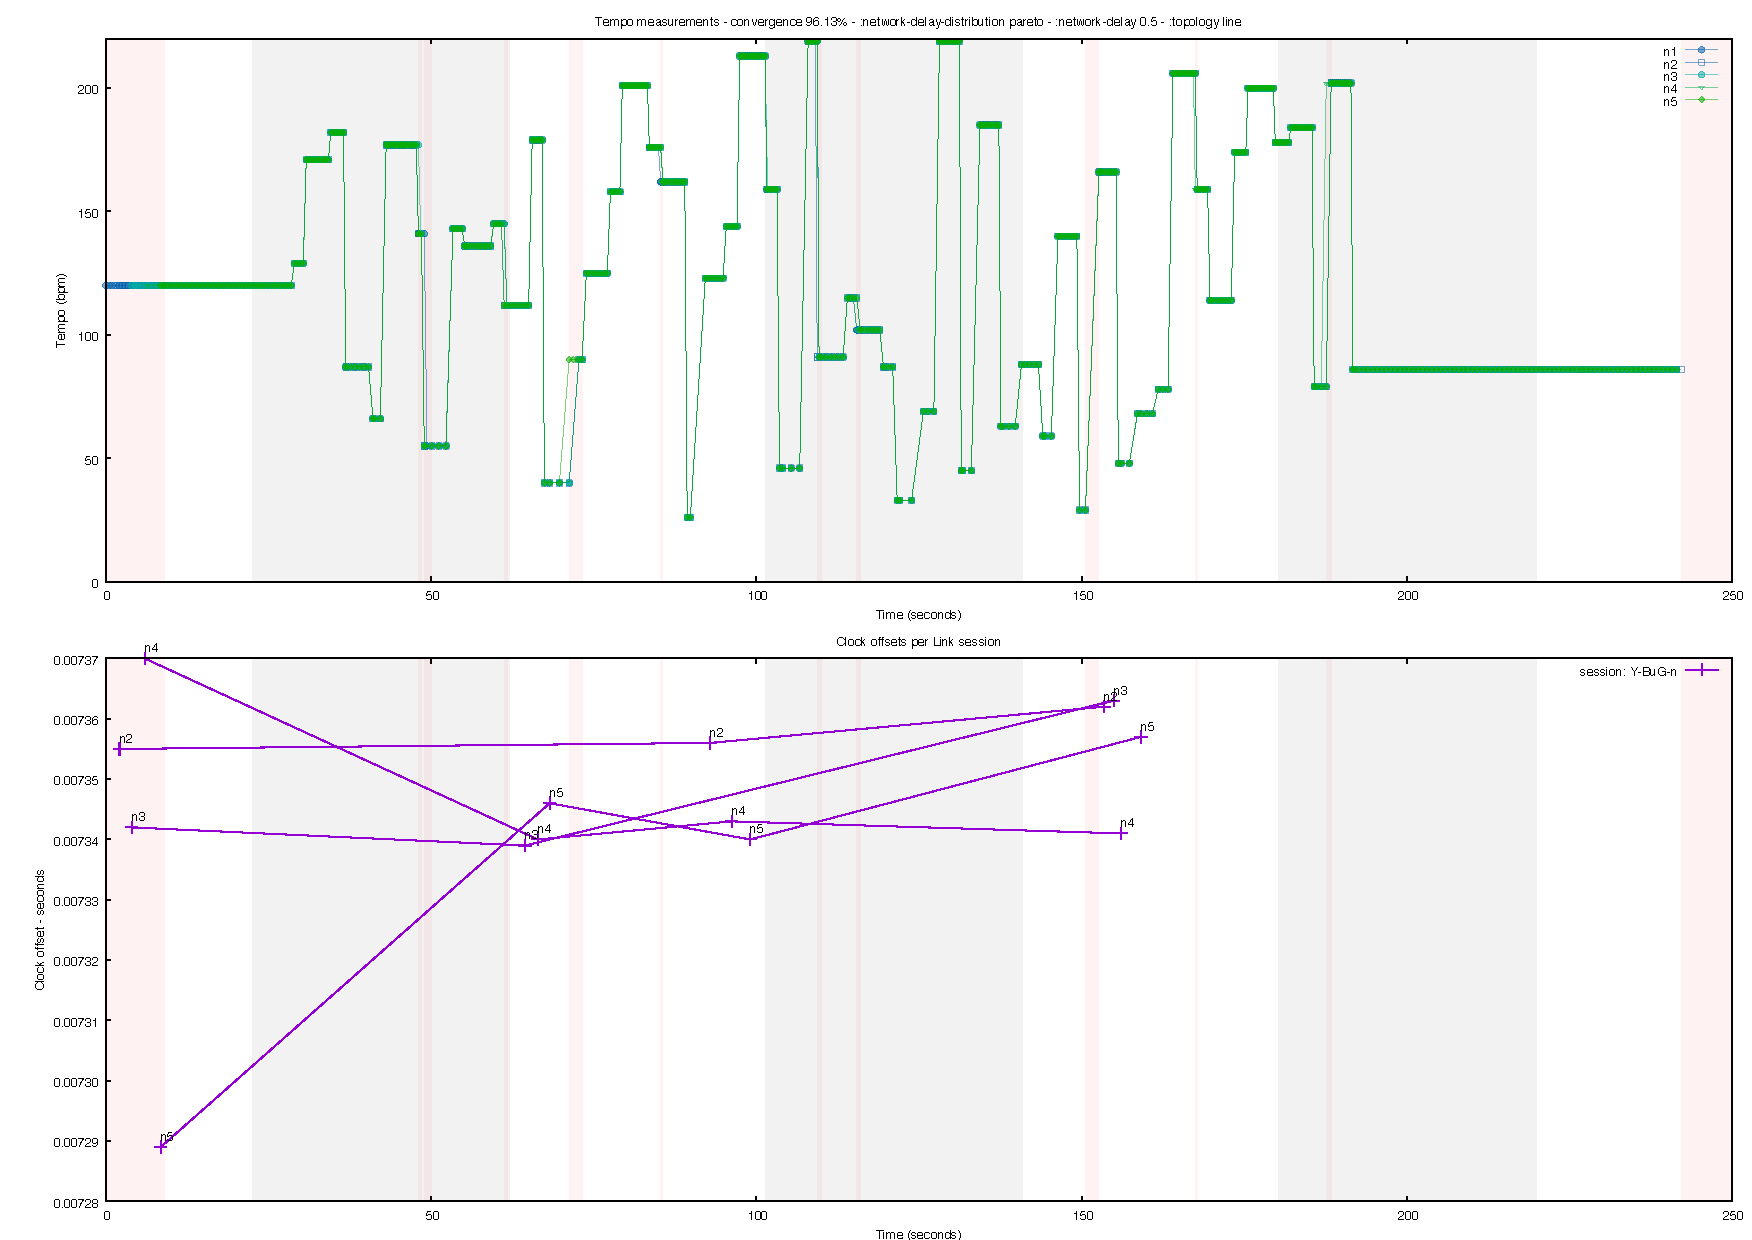
\includepdf[pages=-,angle=-90]{figures-for-publication/tempo_measurements_convergence_96_13_network_delay_distribution_pareto_network_delay_0_5_topology_line/plot.pdf}

\section{Self assessment}

The focus of this work was distilled over time, however the original impetus
was related to my work on the open source music software Sonic
Pi\cite{sonicpi}. From an initial desire to add collaboration features to the
software I began to explore the problem space. Private correspondence with Sam
Aaron was useful in identifying the separate issues of co-located and
geo-distributed performance.

With a view to implementing a custom solution to the co-located problem
specifically, I began some preliminary designs. During this time I was
introduced to the Ableton Link library which articulated many of the ideas I
had already been considering, albeit with greater clarity and focus. As I began
to investigate the Link library I became convinced that it was a well thought
out solution to the co-located problem.

This led to preliminary work with the Link C++ library and as part of this
project I began work on integrating this with the Ruby programming language
(see code listings). Ruby was chosen as this is the primary development
language for Sonic Pi and the creation of a wrapper should be of use in future
integration work.

Many more hours were then spent working out how to instrument the Link codebase
to allow for testing. With very few configuration options, the only path
became to enable and parse the debug logs for information regarding clock
synchronization events. These were largely undocumented meaning that
considerable time was spent on this stage in understanding the output.

With the C++ wrapper written, work moved on to setting up the tests in Jepsen.
This was aided by generally excellent documentation on the Jepsen project,
however the existing examples assumed the use of database client libraries
which meant that working out how to handle more simple connection methods was a
little more opaque.

Jepsen is written in Clojure which meant working in three quite different
languages to produce this work (the others being C++ and Ruby). This was the
source of some cognitive overhead which on reflection was not ideal, but given
the choice again I would still work with the same libraries to do this kind of
testing. I enjoyed working with Clojure and Jepsen in particular and I hope to
work with these to devise more tests in future.

It is with some regret that only a single library was under test in this work,
however after examining various solutions in the same space none of these were
suitable for various reasons. These included reliance on a single operating
system (OS X in the case of Landini\cite{narveson2013landini}), or the need for
graphical interfaces in the case of LNX Studio\cite{lnxstudio}.

The final, and most significant, stage was spent in producing readable output
from which to derive results. Inspiration was taken from the existing
GNU Plot figures that are included with Jepsen to chart network performance,
however all the code to produce the examples in figures here had to be written
from scratch.

When dealing with parsing any text format, issues occur around the quality of
the data. As a result the code contains a lot of incidental complexity which
reflects the fact that the debug logs weren't written with instrumentation in
mind. This has given me some insight into how one might choose to instrument a
similar codebase in future, to aid accurate testing.

Finally while initial drafts of the work focused on variations in topology and
delay, following advice from my supervisor I took the time to investigate
different distributions of delays. This also highlighted to me the surprising
(to me, at least) behaviour of the clock synchronization under symmetric
delays. This meant that further work on the tests was required to ensure that a
consistent leader was chosen for each test run and that delays were only
applied to outbound packets on other nodes.

While the results presented here are not groundbreaking, I do hope that by
offering a practical set of criteria and test bed that it will aid further
research in this area. Thorough analysis of any distributed system is a
difficult task and I have learnt a great deal about this process as a result.

\section{Running the tests}

\begin{minted}{bash}
# clone project and note the path
git clone https://github.com/xavriley/jepsen-ableton-link.git

# clone the Jepsen project to another folder
git clone https://github.com/jepsen-io/jepsen.git#0.1.9
cd jepsen/docker
export JEPSEN_ROOT="/path/to/jepsen.link" # as noted above
./up.sh --dev

# in another window
docker exec -it jepsen-control bash
# once the container has booted
lein run test --time-limit 180 --no-teardown \
--topology line --network-delay 0.5 \
--nemesis-duration 30 --network-delay-distribution constant
\end{minted}

Once that has completed, run the following in the root of the jepsen.link
project:

\begin{minted}{bash}
ruby tempo-grapher.rb
\end{minted}

This will generate the graphs in

\begin{minted}{bash}
./figures_for_publication/_name_of_autogenerated_test_output_directory_/plot.pdf
\end{minted}

following each test run.

\section{Code listings}

The following sections outline the code written in support of this work.

\subsection{\texttt{ruby\char`_ableton\char`_link} gem}

The code is available at
\texttt{https://github.com/xavriley/ruby\char`_ableton\char`_link}.

The majority of interest is contained in the
\texttt{\detokenize{ext/ableton_link/ableton_link.cpp}} file. This contains the
wrapper code for the Ableton Link C++ library.

The wrapper is implemented using the Rice project which provides convenience
functions for interoperability between C++ and Ruby codebases:
\texttt{\detokenize{https://github.com/jasonroelofs/rice}}

The file used for the test procedure is \texttt{bin/server} which contains a
simple TCP server to receive messages containing tempo information while
printing the status of the session on each beat.

\subsection{\texttt{jepsen.link}}

The code is available at
\texttt{https://github.com/xavriley/jepsen-ableton-link}.

This is a Clojure project, using the Jepsen framework. All code relating to the
testing is contained in the \texttt{src/jepsen/link.clj} file.

To produce the graphs the \texttt{tempo-grapher.rb} file is used. This code is
all related to the parsing of log files and the production of a
\texttt{gnuplot} command. The data produced by the parsing is saved to files
and copied to the output directory in case further analysis is required.

\section{Professional issues}

When assessing software solutions for synchronizing musical time, it is
admirable that Ableton Link attempts to do so using permissive licensing and a
committment to cross platform support. In doing so they allow for the
possibility that freely available software may be used for music production
without onerous requirements on the user to learn a particular programming
language or maintain a specific environment in order to be productive. I would
hope that this has a democratizing effect on the landscape for music
production, particularly with regard to some of the academic software output in
this field. These shared projects, while excellent in many respects, often have
a high barrier to entry that musicians with a lack of appropriate resources
would struggle to overcome.

Without more effort on the part of publically funded institutions to target a
non-academic userbase, the danger is for a tendency toward an implicit elitism
in their outputs. Software and music is then written for, and received by,
audiences from within the institutions without regard to how the public life of
the wider communities can be enriched.

With a void of accessible, open source (OSS) alternatives the space is left for
private companies and individuals to "productize" the work done in academia,
with high costs for the end user. Music forms a hobby (in many cases a passion)
among a large percentage of the population - indeed a \textit{dislike} of music
is so rare that it is deemed a medical condition - \textit{musical anhedonia} -
affecting around 3-5\% of the population. Within the rest of the
population exist a large group who invest a great deal of time and energy into
music production. Given the dominance of the private market in digital music
software, this often entails a financial investment too and a dependence on
expensive tools.

Instead of using a passion for digital music making in a constructive way,
proprietary software has no incentive to educate the end user beyond making
them comfortable with their proprietary interface. Music has offered a
gateway into computer science for many current practioners (annecdotally, the
creator of Clojure Rich Hickey started as a music graduate programming
applications for the Atari ST) - if the programming opportunities are not
provided then it's possible that a generation of potential programmers will
miss out on these opportunities.

To this end, open source projects like Sonic Pi\cite{sonicpi} are aiming to
bridge this gap by targetting school children alongside professional users. It
does so by packaging the work of other OSS projects such as SuperCollider, Qt,
QScintilla and the Ruby programming language into a cross-platform environment
with a wide reach and a large userbase. My own contributions to that project
have been with the aim of making new tools of expression more freely available
to those with an interest in creating.

This is where the model of Ableton Link, despite being written by a proprietary
software company, is forward looking in the creation of an open standard to
solve the issue of synchronization.

\section{Acknowledgements}

I would like to record my thanks to a number of groups and individuals, without
whom this work would not have been possible.

Firstly, to the open source community and in particular the Ruby and Clojure
projects and practicioners I have interacted with. These opportunities have
enriched my career immeasurably. In particular I'd like to thank Sam Aaron for
his insightful comments, stimulating discussions and boundless energy in
working on Sonic Pi, along with the other contributors.

It's also fitting that the Kyle Kingsbury's work on the Jepsen project first
piqued my interest in distributed systems, so I'm pleased and proud to have
been able to continue that in the presented work. Honourable mentions also go
to Ableton for developing Link and doing such a good job of it, along with
gnuplot and vimlatex for making the test results look half decent.

My thanks also to my work colleagues at Heroku for supporting me during a
part-time pursuit of a Masters degree and to Salesforce for the generous
funding policy.

To Gregory and the teaching staff at RHUL, I'm forever grateful that I was
given the opportunity to study with you and I've found it rewarding and
challenging in the best possible way.

Finally, to my friend David Bamber for introducing me to the idea that
programming was for me, to my family for unerring support and to my wife Em who
has been consistent, persistent and fault tolerant throughout.

\end{document}
